\documentclass[letterpaper, 11pt]{article}
\usepackage{amsmath}
\usepackage{amssymb}
\usepackage{float}
\usepackage{inputenc}
\usepackage[left=2cm, right=2cm, top=2cm, bottom=2cm]{geometry}
\usepackage{graphicx}
\usepackage{float}
\usepackage{caption}
\usepackage{extarrows}
\usepackage{xcolor}
\usepackage{lscape}
\usepackage{pdflscape}
\usepackage{pdfpages}
\usepackage{multicol}
\usepackage{leftindex}
\usepackage{algorithm2e}
\SetKwComment{Comment}{/* }{ */}
%\RestyleAlgo{ruled}
\usepackage{mathtools}
\usepackage{hyperref}
\hypersetup{
    colorlinks=false,
    }

% Listings
\usepackage{listings}
\usepackage{color}
\definecolor{mygreen}{rgb}{0,0.6,0}
\definecolor{mygray}{rgb}{0.5,0.5,0.5}
\definecolor{mymauve}{rgb}{0.58,0,0.82}

\lstset{
  backgroundcolor=\color{white},   % choose the background color; you must add \usepackage{color} or \usepackage{xcolor}; should come as last argument
  basicstyle=\small\ttfamily,        % the size of the fonts that are used for the code
  breakatwhitespace=false,         % sets if automatic breaks should only happen at whitespace
  breaklines=true,                 % sets automatic line breaking
  captionpos=t,                    % sets the caption-position to bottom
  commentstyle=\color{mygreen},    % comment style
  deletekeywords={...},            % if you want to delete keywords from the given language
  escapeinside={\%*}{*)},          % if you want to add LaTeX within your code
  extendedchars=true,              % lets you use non-ASCII characters; for 8-bits encodings only, does not work with UTF-8
  firstnumber=1,                % start line enumeration with line 1000
  frame=false,	                   % adds a frame around the code
  keepspaces=true,                 % keeps spaces in text, useful for keeping indentation of code (possibly needs columns=flexible)
  keywordstyle=\color{blue},       % keyword style
  language=Python,                 % the language of the code
  morekeywords={*,...},            % if you want to add more keywords to the set
  numbers=none,                    % where to put the line-numbers; possible values are (none, left, right)
  numbersep=5pt,                   % how far the line-numbers are from the code
  numberstyle=\tiny\color{mygray}, % the style that is used for the line-numbers
  rulecolor=\color{black},         % if not set, the frame-color may be changed on line-breaks within not-black text (e.g. comments (green here))
  showspaces=false,                % show spaces everywhere adding particular underscores; it overrides 'showstringspaces'
  showstringspaces=false,          % underline spaces within strings only
  showtabs=false,                  % show tabs within strings adding particular underscores
  stepnumber=5,                    % the step between two line-numbers. If it's 1, each line will be numbered
  stringstyle=\color{mymauve},     % string literal style
  tabsize=4,	                   % sets default tabsize to 2 spaces
  title=\lstname                   % show the filename of files included with \lstinputlisting; also try caption instead of title
}


% NewCommands
\newcommand{\peq}{ \mathrel{+}= }
\newcommand{\muleq}{ \mathrel{*}= }
\newcommand{\sign}{\,\text{sign}}
\newcommand{\bm}[1]{\begin{bmatrix} #1 \end{bmatrix}}
\newcommand{\lx}[2]{\leftindex #1 {#2}}
\newcommand{\norm}[1]{\left\lvert #1 \right\rvert}
\newcommand{\abs}[1]{\norm{#1}}
\newcommand{\itbf}[1]{\textit{\textbf{#1}}}
\newcommand{\mdet}[1]{\norm{\begin{matrix} #1 \end{matrix}}}
\newcommand{\lr}[1]{\left( #1 \right)}
\newcommand{\sat}{\,\text{sat}}



\title{Identification and Control of Multirotor Actuator Dynamics with RPM feedback}
\author{Sesha Charla}
\date{\today}


\begin{document}
\maketitle
\tableofcontents
%===============================================================================
\newpage
\part{Model Parameter Identification}
\section{Brushless DC motor model}
\subsection{Brushless DC motor speed-troque characteristics \cite{crowder2019electric}}
The torque and speed characteristics can be determined by the balance between motor's mechanical output power adn electrical input power over a conduction period:
\begin{align*}
    P &= \omega_m T_e = 2 e_p I\\
    e_p &= N_p B_g \pi r l \omega_m\\
    \text{Where, } \qquad &\\
    \omega_m &- \text{Mechanical rpm}\\
    T_e      &- \text{Electromagnetic torque}\\
    e_p      &- \text{Back emf}
\end{align*}

The factor 2 is the result of current flowing through 2-motor phases (trapesoidal wave form).\\

We have, electromagnetic torque:
\begin{align*}
    T_e &= 4 N_p B_g l r I &[\because \text{Lenz law}]
\end{align*}
let, $E = 2 e_p$. We have,
\begin{align*}
    E &= k \psi \omega_m = K_v \omega_m\\
    T_e &= k \psi I = K_T I\\
\text{Where, } \qquad &\\
    k &= 4 N_p  &(\text{Armature Constant})\\
    \psi &= B_g \pi  r l  &(\text{Flux})
\end{align*}

Thus, ideally back-emf constant and torque constants are same.\\

Using the above equations, the following steady-state torque speed characteristics can be drived. We have, the instantaneous voltage equation:
\begin{align*}
    V_s &= E + I R\\
\text{Where, } \qquad &\\
    V_s &- \text{Supply voltage}\\
    I &- \text{Total DC current}\\
    R &- \text{Sum of the terminal phase ressistances}
\end{align*}

We have torque speed relationship:
\begin{align*}
    \omega_m &= \omega_0 \left( 1 - \frac{T}{T_0} \right)\\
\text{Where, } \qquad &\\
    \omega_0 &= \frac{V_s}{k \psi} & (\text{No-load Speed})\\
    T_0 &= k \psi I_0              & (\text{Stall Torque})\\
    I_0 &= \frac{V_s}{R}           & (\text{Stall Current})
\end{align*}

\subsection{Dynamic Model (without Propeller)}
We have the dynamic model of BLDC motor using moment balance:
\begin{align*}
    J_m \dot \omega_m &= T_e - b_f \omega_m - M_f\\
    \text{where, } \qquad &\\
    J_m &- \text{Moment of inertia of the motor}\\
    b_f &- \text{lumped parameter for viscous friction}\\
    M_f &- \text{lumped parameter for coulomb friction}
\end{align*}
\itbf{Friction:}
\begin{enumerate}
    \item Viscous friction: $-b_f \omega$.
    \item Columb friction: $-M_{f} \sign(\omega) = -M_{f} \qquad [\because$ the motor turns in only one direction $]$.
\end{enumerate}

\medskip

From the speed-torque characteristics of the BLDC motor:
\begin{align*}
    T_e &= K_T I = K_T \frac{(V_s - E)}{R} = \frac{K_T}{R} (V_s - K_v \omega_m)  & [\because K_v = K_T = k \psi]\\
    \text{Let, }\qquad \qquad &\\
    K_r &= \frac{K_T}{R}
\end{align*}
From the definition of Input to ESC:
\begin{align*}
    V_s &= u V_{in}\\
    \therefore T_e &= u K_r V_{in} - K_r K_v \omega_m
\end{align*}

Substituting:
\begin{align*}
    &J_m \dot \omega_m = u K_r V_{in}  - K_rK_v \omega_m  - b_f \omega_m - M_f
\end{align*}
\begin{equation}
    \boxed{
    J_m \dot \omega_m + (K_r K_v  + b_f) \omega_m + M_f = u K_r V_{in}
    }
    \label{eqn:no_prop}
\end{equation}

\subsection{BLDC Motor with Propeller}
Adding propeller moment of inertia and the moment due to propeller drag into the BLDC motor model.
\begin{align*}
    (J_m + J_p) \dot \omega + (K_rK_v + b_f) \omega + M_f &= u K_r V_{in} - C_D \omega^2
\end{align*}
Where, $C_D$ is the aerodynamic drag. Let, $J_m + J_p = J$
\begin{equation}
    \boxed{
    J\dot \omega + (K_rK_v + b_f) \omega + C_D \omega^2 + M_f = u K_r V_{in}
    }
    \label{eqn:prop}
\end{equation}


%    \text{Substituting, } \quad K_r u &= (K_r K_v  + b_f) u_\omega + \frac{M_f}{\hat V_{in}}\\
%   J\dot \omega + (K_rK_v + b_f) \omega + C_D \omega^2 + M_f &= V_{in} \left((K_r K_v  + b_f) u_\omega + \frac{M_f}{\hat V_{in}} \right)\\



% \begin{align*}
%     \text{Using normalized no-load angular velocity input:} &\\
%     J_m \dot \omega_m + (K_r K_v  + b_f) \omega_m + M_f &= \left(\left(\frac{K_r K_v  + b_f}{K_r} \right) u_{\omega} + \frac{M_f}{K_r \hat V_{in}} \right) K_r V_{in}\\
%     &= V_{in}(K_r K_v  + b_f)u_{\omega} + M_f \frac{V_{in}}{\hat V_{in}}
% \end{align*}

% We get the linearised model using small perturbtation:
% \begin{align*}
%     J_m \delta \dot \omega_m + (K_rK_v + b_f) \delta  \omega_m  &= \delta u_{\omega}V_{in}(K_r K_v  + b_f) \\
%     \frac{\delta \omega_m (s)}{\delta u (s)} &= \frac{V_{in}(K_r K_v  + b_f)}{J_m s + (K_r K_v + b_f)} = \frac{V_{in}}{\frac{J_m}{(K_r K_v + b_f)} s + 1} = \frac{K_m}{\tau_m s + 1}\\
%     \text{where, }\qquad &\\
%     K_m &= V_{in}\\
%     \tau_m &= \frac{J_m}{(K_rK_v + b_f)}
% \end{align*}

% \begin{minipage}{0.49\textwidth}
% Writing interms of $\delta u_p$:
% \begin{align*}
%    \delta u_\omega &= g'_w(u_p) \delta u_p\\
%    \implies \frac{\delta \omega_m (s)}{\delta u_{p} (s)} &= \frac{K g'_w(u_p)}{\tau s + 1}
% \end{align*}
% This explains the static gain variation observed in the system identification.
% \end{minipage}
% \begin{minipage}{0.49\textwidth}
%  \begin{figure}[H]
%     \centering
%     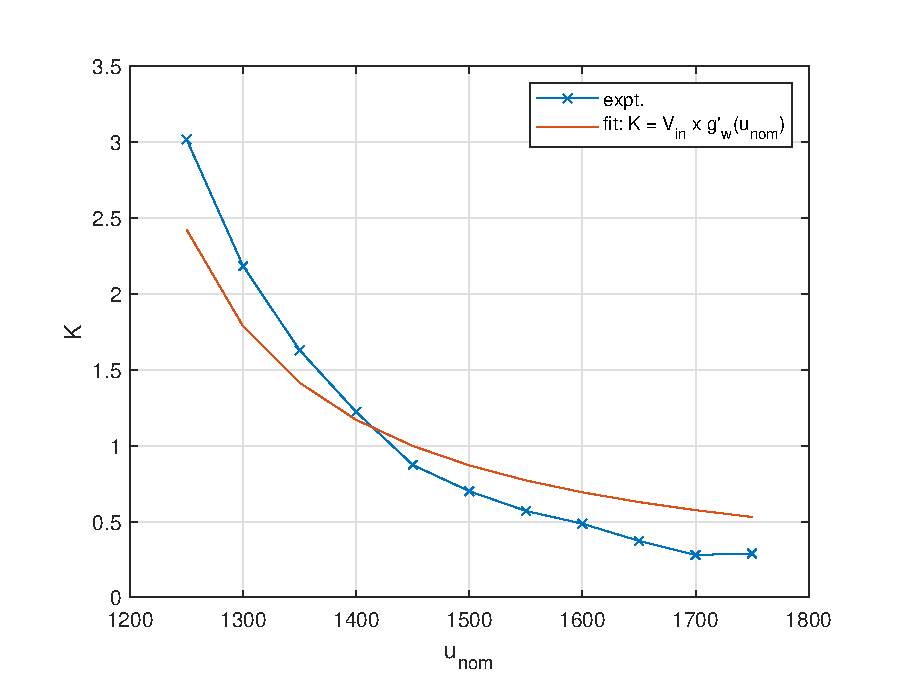
\includegraphics[width = \textwidth]{./figs/norm_omega/K_fit.eps}
%     \caption{Static gain variation with nominal input ($u_p$) with input perturbtation $\delta u_p = 100 \mu s$}
% \end{figure}
% \end{minipage}
% %===============================================================================
%\subsection{Parametric Identification model for BLDC motor dyanmcis}
%\subsubsection{Continuous Parametric Model}
%\begin{align*}
%    J_m \dot \omega &= -(K_rK_v + b_f) \omega_m - M_f + u K_r V_{in}\\
%   %===
%    \implies \dot \omega &= -\frac{(K_rK_v + b_f)}{J_m} \omega_m - \frac{M_f}{J_m} + u \frac{K_r V_{in}}{J_m}
%\end{align*}
%
%Hence, we have the continuous parametric model:
%$$ \dot \omega =
%    \underbrace{\begin{bmatrix}
%               - \omega  & -1
%\end{bmatrix}}_{\Phi^T(\omega)}
%\underbrace{\begin{bmatrix}
%    \frac{(K_rK_v + b_f)}{J_m}  \\
%    \frac{M_f}{J_m}
%\end{bmatrix} }_{\pmb \theta}
%    +\frac{K_r V_{in}}{J_m}u $$
%
%Let,
%\begin{align*}
%    a_1 &= \frac{(K_rK_v + b_f)}{J_m} \qquad
%    a_2 =   \frac{M_f}{J_m}\\
%    \\
%    \pmb \theta &= \begin{bmatrix}a_1 & a_2 \end{bmatrix}^T \qquad
%    b =  \frac{K_r V_{in}}{J_m}
%\end{align*}
%
%$$\therefore \dot \omega = \Phi^T(\omega) \pmb \theta + b u$$
%
%\subsubsection{Descritezed Parametric Model}
%Descritizing the above model using euler-method $\left(\dot \omega = \frac{\omega[k] - \omega[k-1]}{h}\right)$, with $h$ as the sampling interval:
%
%\begin{align*}
%    \frac{\omega[k] - \omega[k-1]}{h} &=
%    \begin{bmatrix}  - \omega[k-1]  &  -1 \end{bmatrix}
%    \begin{bmatrix}
%        a_1 \\ a_2
%    \end{bmatrix}
%    + bu[k-1]\\
%    %===
%    \omega[k] &= h \begin{bmatrix} - \omega[k-1]  & -1 \end{bmatrix}
%    \begin{bmatrix}
%        a_1 - \frac{1}{h} \\
%        a_2 \\
%    \end{bmatrix}
%    + b  h u[k-1]\\
%    %===
%    &= h \begin{bmatrix} -\omega[k-1] & -1 & u[k] \end{bmatrix}
%    \begin{bmatrix}
%        a_1 - \frac{1}{h} \\
%        a_2 \\
%        b
%    \end{bmatrix}
%\end{align*}
%
%Let,
%\begin{align*}
%    \pmb \theta_h = h
%    \begin{bmatrix}
%        a_1 - \frac{1}{h} \\
%        a_2 \\
%        b
%    \end{bmatrix} =
%    h
%    \begin{bmatrix}
%        \frac{(K_rK_v + b_f)}{J_m} - \frac{1}{h}  \\
%        \frac{M_f}{J_m}\\
%        \frac{K_r V_{in}}{J_m}
%    \end{bmatrix}
%    \qquad \text{and} \qquad
%    \Phi(\omega[k-1], u[k])^T &=  \begin{bmatrix}  -\omega[k-1] & -1 & u[k-1] \end{bmatrix}
%\end{align*}
%
%hence, we have the parametric model in least-squares form:
%\begin{align*}
%    \omega[k] &= \Phi(\omega[k-1], u[k-1])^T \pmb \theta_h
%\end{align*}
%

\subsection{Propeller Aerodynamics}
Aerodynamics are assumed to be faster than mechanical dynamics of the actuator.
The thrust generation process due to the propagation of pressure wave is assumed to be instantaneous. This assumption is inherent to the standard models that use potential flow theory (lifting-line, blade-element and momentum-disk theories), as they assume incompressible flow.\\

\begin{minipage}{0.49\textwidth}
    \itbf{Propeller Thrust}:
    \begin{align*}
        F_T = C_{T} \omega^2
    \end{align*}

    \itbf{Propeller moment due to drag}:
    \begin{align*}
        M_D = C_{D} \omega^2
    \end{align*}
\end{minipage}
\begin{minipage}{0.49\textwidth}
    \begin{figure}[H]
        \centering
        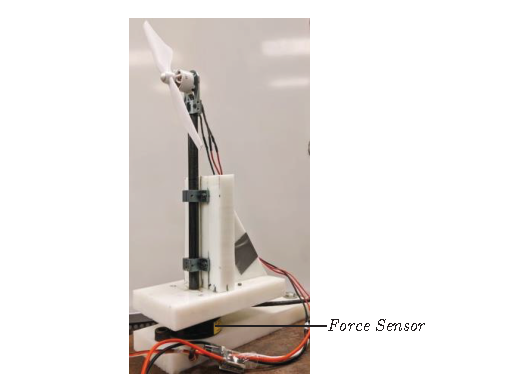
\includegraphics[width = \textwidth]{figs/aero/expt_setup.eps}
        \caption{Experimental Setup}
        \label{fig:expt_setup}
    \end{figure}
\end{minipage}

\bigskip

\textbf{Aeroelasticity of the propeller:} It is assumed that the aeroelasticity of the propeller produces high-frequency oscillations in the thrust and torque of the propller which are assumed to be very fast and roll off w.r.t the mechanical dyanmics dyanmics of the actuator as well as the transmission through the propller shaft. The constant  bias in the torque due to flutter is captured in the drag coefficient and it's parameter uncertainity.\\


\subsubsection{Parameter estimation form the static data}

In the experimental setup (Figure~\ref{fig:expt_setup}),  the total moment measured is the result of aerodynamic moment and the friction of the BLDC motor. Thus the total moment becomes:
\begin{align*}
    M = C_D \omega^2 + b_f \omega + M_f
\end{align*}

The aerodynamic coefficients are estimated from the static measuremnts using least-squares estimation.

\begin{figure}[H]
    \begin{minipage}{0.49\textwidth}
        \begin{figure}[H]
            \centering
            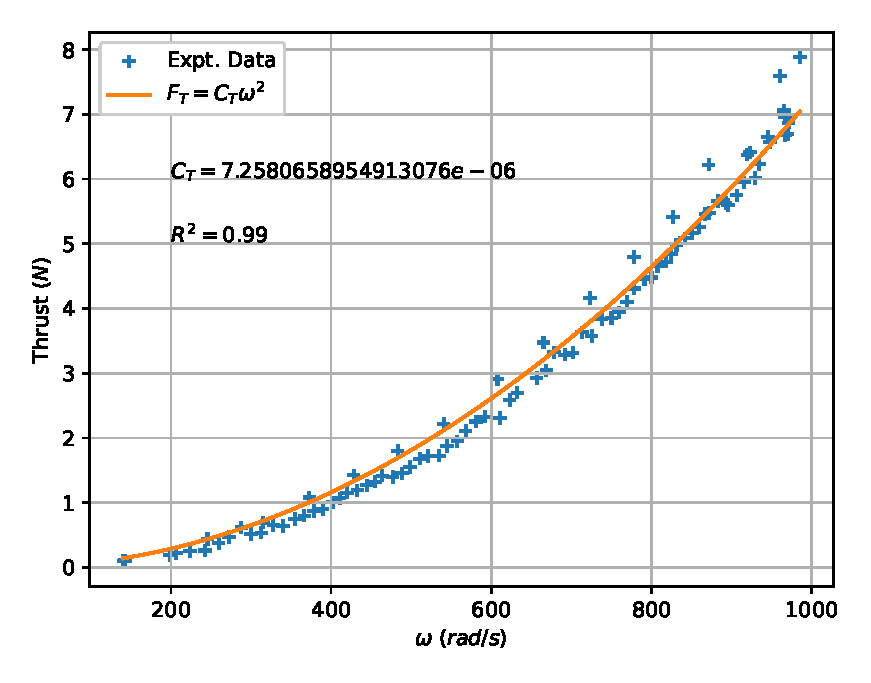
\includegraphics[width = \textwidth]{./figs/aero/Thrust_curve.eps}
        \end{figure}
        \caption{Variation of thrust with rpm}
    \end{minipage}
    \begin{minipage}{0.49\textwidth}
        \begin{figure}[H]
            \centering
            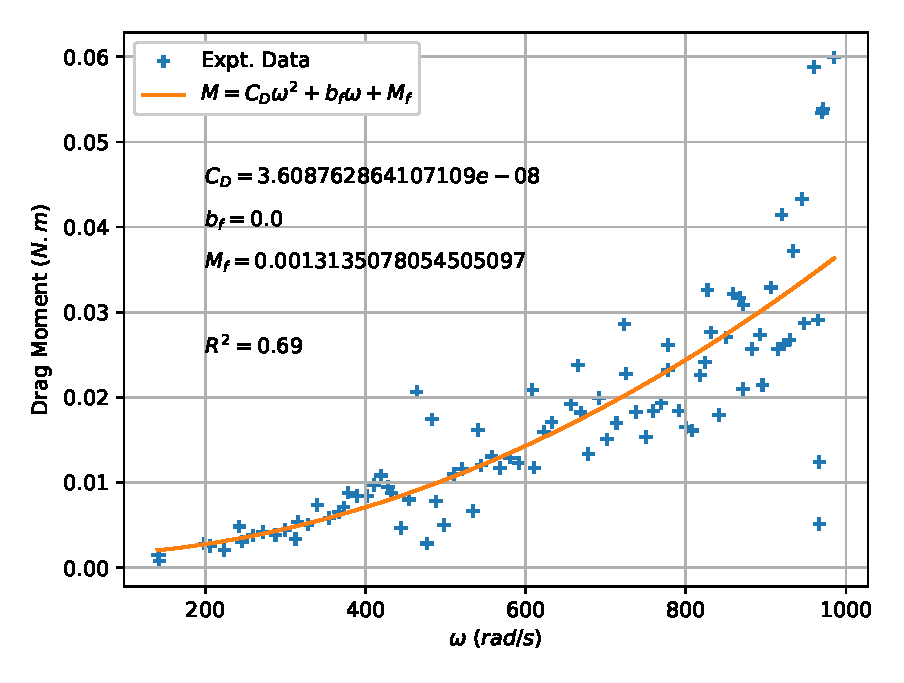
\includegraphics[width = \textwidth]{./figs/aero/Drag_curve.eps}
            \caption{Variation of drag moment with rpm}
        \end{figure}
    \end{minipage}
\end{figure}

The moment data has more variation from model due to the unmodelled aerodynamic effects such as aerodynamic-flutter. Thus we have the estimates of force coefficients:

\begin{table}[H]
    \centering
    \begin{tabular}{c l}
        \hline \hline
        Parameter & Value \\ \hline \hline
        $C_T$ & $7.2581 \times 10^{-06}$ $N/(rad/s)^2$  \\
        $C_D$ & $3.6088 \times 10^{-08}$ $N.m/(rad/s)^2$ \\
        $b_f$ & $0.0$ $N.m/(rad/s)$\\
        $M_f$ & $1.3135 \times 10^{-3}$ $N.m$\\ \hline \hline
    \end{tabular}
    \caption{Estimates Force coefficients}
\end{table}

%===============================================================================
\newpage
\section{RPM Measurement}
An is interrupt triggered for every commutation high and the ISR gets the counter
value of an independently runing timer. Using this value, the RPM is calcluated
at every interrupt trigger as follows:
\begin{align*}
    rpm &= \frac{60 f_t}{N_p \times T_c}\\
    \text{Where,} \qquad &\\
    f_t &- \text{Frequency of the timer counts (here, $1$ MHz)}\\
    N_p &- \text{Number of pole-pairs in the BLDC motor (here, $7$)}\\
    T_c &- \text{Timer counts between the two interrupts}
\end{align*}

The above method of measurement is verified against the tach-meter reading. The
readings are in agreement with each other, validating the measurement method.
\begin{figure}[H]
    \centering
    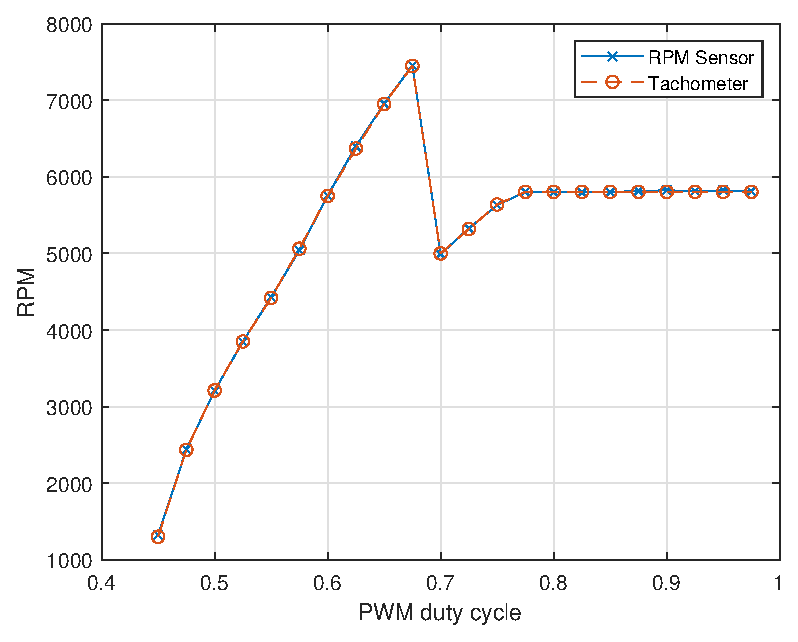
\includegraphics[width=0.5\textwidth]{./figs/rpm_feedback/static_calib.eps}
    \caption{Rpm sensor and tachometer readings}
\end{figure}

The above method has an inherent flow at very low $rpm$s where there is no
commutation at a given sampling instance which results in a zero rpm at that
sample making the sensor noisy. This can be avoided by holding the rpm value
from the previous measurement if there is no commutation in the sample instance.

\bigskip

\itbf{Using external interrupt and  timer}
\par The commutations can be counted using external interrupts. The actual measurement of rpm involves a raising-edge triggered external interrupt and a timer interrupt. The ISR of the external interrupt updates a counter corresponding to the pulses (here, the electrical commutations). The timer-interrupt polls for this counter value at the specified frequency $(f_s)$ and resets the counter. The rpm is calculated from this counter value as follows:
$$rpm = \frac{counter\_value}{N_P} \times f_s \times 60$$
where, \\
$N_p - $ No. poles in the BLDC motor\\

\par The minimum rpm that can be measured depends on the sampling frequency and the poles in the BLDC motor $(= \frac{60f_s}{N_P} )$. And the maximum depends on the clock frequency of the micro-controller as the frequency of interrupts and ISR calls becomes the bottleneck in this case. The resolution of the sensor also depends on the sampling frequency and poles as the counter value is an integer. We have,
$$Sensor \, resolution = \frac{60f_s}{N_P}$$

\par For the current system the range of rpm is $[2000, 10000]$. The number of poles in BLDC motor are $12$. Assuming the acquisition frequency of $400\,Hz$, the resolution for the above sensor will be:
$$Sensor \, resolution = \frac{60f_s}{N_P} = 2000 \, rpm = 209.4395 \, rad/s$$
For $100 \, Hz$ acquisition rate:
$$Sensor \, resolution = 500 \, rpm = 52.3599 \, rad/s$$

\par The main source of sensor noise in this case is the latency of the external interrupt. The counter value will be oscillating around the actual value based on the timing of external and timer interrupts causing the measured rpm to fluctuate. Based on the resolution calculations above, the signal-to-noise ratio of the system will be very high if the current implementation is used. \\

\par This problem of resolution and signal-to-noise ratio is due to the interfacing method used. Alternatively, the following method is propsoed to overcome this problem.

\bigskip

\itbf{Using two timers and an external interrupt}
\par We use and additional timer as a high frequency counter of frequency $f_t$ for calculating the rpm at every sampling period as follows:
$$rpm = \frac{counter\_value \times f_t}{N_P \times time\_counts} \times 60$$
where, \\
$N_p - $ No. poles in the BLDC motor\\
$time\_counts - $ Number of timer interrupt counts during the sampling interval.\\
Hence, we have, maximum number of $time\_counts$ in a sampling interval is $f_s/f_t$\\
$$\implies Sensor \, resolution = \frac{60f_s}{N_P f_t} = rpm_{min}$$
Therefore, the resolution of the sensor can be increased by arbitrarily increasing the frequency of the high frequency counter, limited only by the hardware.\\

For example, if $f_h = 1000\, Hz$, for the same values as above, the resolution of the sensor:
$$Sensor \, resolution = \frac{60f_s}{N_P \times f_t} = \frac{2000}{1000} = 2 \, rpm = \frac{1}{\pi} \, rad/s$$

\par This method will reduce the signal-to-noise ratio significantly.

\subsection{Measurement Algorithm}
\par In higher rpm cases there are more than one measurement instance wthin
the sample time. Median of these measurements can be used to reduce sudden spikes in the data due to interrupts skips. Combining this with
higher resolution algorithm, we have the algorithm for rpm measurement:\\

Let $C_c$ be the current value of the 32-bit timer, $P_c$ the previous value and $n_C$ be the number of commutations within the sample.\\

At every interrupt trigger (in ISR)

    \begin{algorithm}[H]
        $n_C \peq 1$\;
        $\delta t_k = C_c - P_c$\;
        \If{ $\delta t_k \leq 0$ }
            {$\delta t_k \peq 2^{32}$ \Comment*[r]{Correcting for integer overflow}}
        $\pmb{\delta t_k} [n_C-1] =  \delta t_k$\;
        $P_c = C_c$\;
    \end{algorithm}

At every sampling instance (in $get\_rpm()$):

    \begin{algorithm}[H]
        $N_p = 7$\;
        $f_t = 10^6$\;
        $M = \frac{2 \pi}{N_p} \times f_t$\;
        \eIf {$n_C > 0$ and $n_C \leq n_{C_{max}}$ and $\norm{n_C - n_{C_{old}}} \leq \delta n_{C_{max}}$}
            {$\omega = \frac{M}{\text{Median}(\pmb{\delta t_k})}$ \Comment*[r]{Median removes spikes in the data}
             $ \omega_{old} = \omega$\;
             $n_{C_{old}} = n_C$\;
            }
             {$\omega = \omega_{old}$}
        $n_C = 0$\;
        $\pmb{\delta t_k} = \pmb 0$\;
    \end{algorithm}

\begin{figure}[H]
    \begin{minipage}{0.49\textwidth}
        \begin{figure}[H]
            \centering
            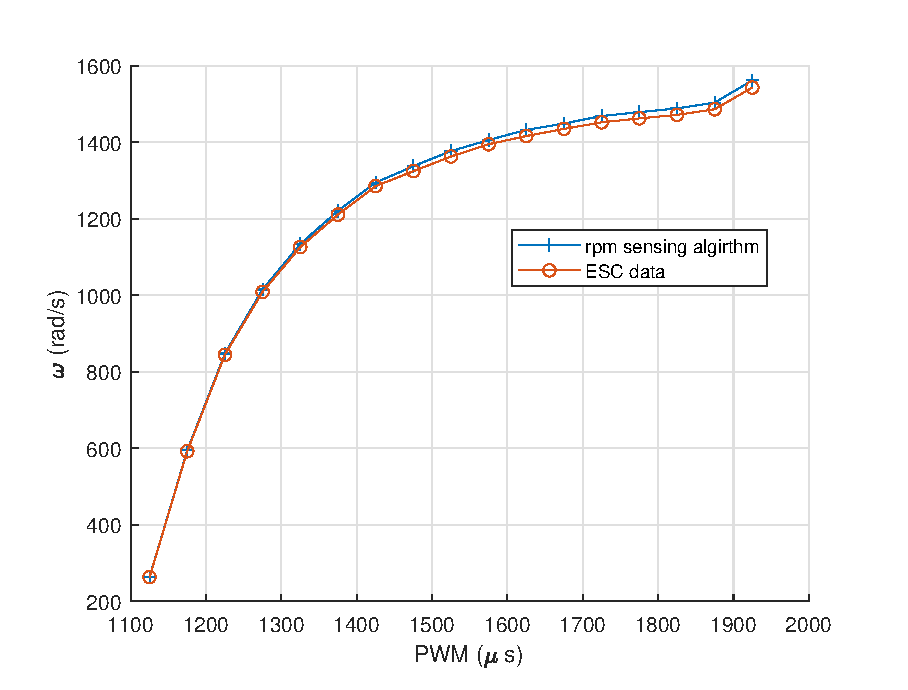
\includegraphics[width = \textwidth]{./figs/rpm_feedback/rpm_meas_noprop.eps}
            \caption*{Without Propeller}
        \end{figure}
    \end{minipage}
    \begin{minipage}{0.49\textwidth}
        \begin{figure}[H]
            \centering
            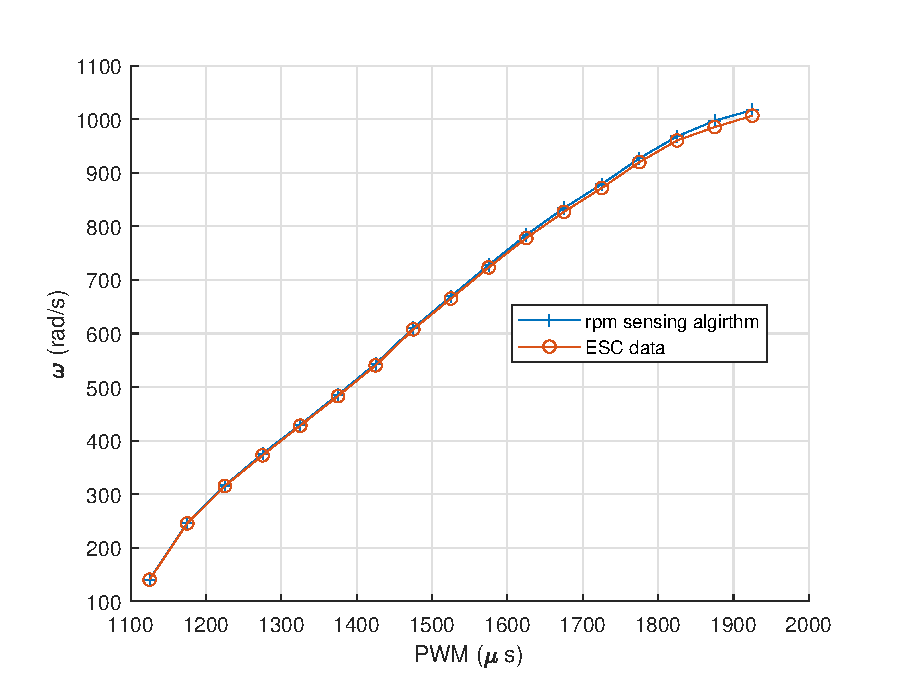
\includegraphics[width = \textwidth]{./figs/rpm_feedback/rpm_meas_prop.eps}
            \caption*{With Propeller}
        \end{figure}
    \end{minipage}
    \caption{Validating the measurement algorithm}
\end{figure}

%===============================================================================
\newpage
\section{Input definition and Static Calibration}
\subsection{ESC and non-linear input compensation}

The castle creations ESC has a micro-controller that non-lineraly scales the input PWM signal's duty-cycle to the duty-cycle of the $24\,kHz -$PWM signals to the inverter effectively scaling the source voltage to the motor by the duty-cycle. This is done to have a linear input to thrust curve instead of a quadratic one.

The input transmission can be described as follows: The $400\,Hz-$PWM duty cycle ($u_p$) islineraly scaled to a throttle ratio $(p)$ ($\%$ power-out) between 0 and 1. Which is then filters using a non-linear function $(g_u)$ to get the PWM duty-cycle input to the inverter ($u$) \cite{kim2017electric}.

\begin{align*}
    u_p \rightarrow \boxed{g_u(.)} \rightarrow u
\end{align*}
and finally,
$$V_s = u V_{in} \qquad u \in [0, 1]$$

$u$ is considered as the input to the motor-propeller system and the necessary invertion will be performed for transmitting the signals.

\itbf{Scaling PWM Singal Duty cycle based on switching frequency}:
Pixhawk-4 uses a switching frequency of $400\,Hz$ for its PWM signals (can be swithed to $50 \, Hz$ which is not that usefull in case of BLDC motors but usefull for servos). The controller thus scales the PWM duty cycle to the duration of on-time of the signal in its period in 'microseconds'. These inputs are handelled as integer types within the range [800, 2200]\cite{px4_pwm}.

The current ESC that has the rpm-feedback capabilites has an operating range between $1110 \, \mu s$ and $1890 \, \mu s$. After that, the ESC switchs to a constant power mode which sets the rpm to a constant.
\begin{align*}
    \text{Period of the PWM wave } &= \frac{1}{400} \times 10^6 \, \mu s = 2500 \, \mu s\\
    \text{Minimum Operating Duty Cycle } &= \frac{1110}{2500} = 0.444\\
    \text{Maximum Operating Duty Cycle } &= \frac{1890}{2500} = 0.756\\
\end{align*}

$u$ can be considered to be the actual input to the system and system identification with the propeller. It turns out that the parameters of the above non-linear filter are not estimatable with the give information. To solve this problem, we chose angular velocity of the motor with propeller normalized with voltage as the input instead.

\subsection{Normalized No-load Angular Velocity Input}

We have the no-load dynamic model for the BLDC motor:
\begin{align*}
    J_m \dot \omega_m + (K_r K_v  + b_f) \omega_m + M_f &= u K_r V_{in}
\end{align*}
At steady state ($\dot \omega_m = 0$), the above equation becomes:
\begin{align*}
    (K_r K_v  + b_f) \omega_m + M_f &= u K_r V_{in}
\end{align*}
Substituting the non-linear input filter:
\begin{align*}
    (K_r K_v  + b_f) \omega_m + M_f &= g_u(u_p) K_r V_{in}\\
    \implies \frac{(K_r K_v  + b_f)}{K_r} \left(\frac{\omega_m}{V_{in}}\right) + \frac{M_f}{K_r V_{in}} &= g_u(u_p)
\end{align*}

\itbf{Definition}: Let, $u_{\omega}$ be the no-load angular velocity of the motor at unit supply voltage for the given pwm input ($u_p$). Also, let us call it "\itbf{Normalized no-load angular velocity}".
\begin{align*}
    u_{\omega} &= \frac{\omega_m}{V_{in}} \text{  at  } u_p
\end{align*}
Thus,
\begin{align*}
    \left(\frac{K_r K_v  + b_f}{K_r} \right) u_{\omega} &+ \frac{M_f}{K_r V_{in}} = g_u(u_p)\\
    \implies u_{\omega} &= \left(\frac{K_r}{K_r K_v  + b_f} \right) \left( g_u(u_p) - \frac{M_f}{K_r V_{in}} \right)\\
    &= \left(\frac{K_r}{K_r K_v  + b_f} \right) g_u(u_p) - \left(\frac{1}{K_r K_v  + b_f} \right) \frac{M_f}{V_{in}}
\end{align*}
Assuming, the supply voltage will not be varying much and the variation will be captured in the input uncertainity. Let $V_{in}$ on the RHS be $\hat V_{in}$. thus:
\begin{align*}
    u_{\omega} &= \left(\frac{K_r}{K_r K_v  + b_f} \right) g_u(u_p) - \left(\frac{1}{K_r K_v  + b_f} \right) \frac{M_f}{\hat V_{in}}
\end{align*}
Let,
\begin{align*}
    g_w (u_p) &= \left(\frac{K_r}{K_r K_v  + b_f} \right) g_u(u_p) - \left(\frac{1}{K_r K_v  + b_f} \right) \frac{M_f}{\hat V_{in}}
\end{align*}
The parmeters of assumed structure of $g_w(.)$ are estimatable form the experimental data ($\omega, u_p$) unlike $g_u$. Though, this method introduces additional uncertainity because of the $\hat V_{in}$, but it can be justifiably assumed to be far less than the uncertainity due to fitting ($\omega-u_p$) curve with for $g_w(.)$.

Writing, $u_{\omega}$ interms of actual PWM input to the motor $u$.
\begin{align*}
    u_{\omega} &= \left(\frac{K_r}{K_r K_v  + b_f} \right) u - \left(\frac{1}{K_r K_v  + b_f} \right) \frac{M_f}{\hat V_{in}}
\end{align*}
\begin{equation}
    \implies K_r u = (K_r K_v  + b_f) u_\omega + \frac{M_f}{\hat V_{in}}
    \label{eqn:norm_in}
\end{equation}
Thus, $u_{\omega}$ is $u$ scaled lineraly.

\subsubsection{Logarithmic form for $g_w(.)$ and Parameter Estimation}

Based on the experimental data, $g_w(.)$ is assumed to have the following logarithmic (natural-log) form:
\begin{align*}
    g_w(u_p) &= a \ln(u_p - 1110) + b
\end{align*}
The choice of bias as $1110$ was due to the fact that the maximum input that can be given to the esc-motor sytem with no response is 1110. The values of $a, b$ are obtained by lineraly fitting $u_\omega$ to $u_p$.

\begin{figure}[H]
    \centering
    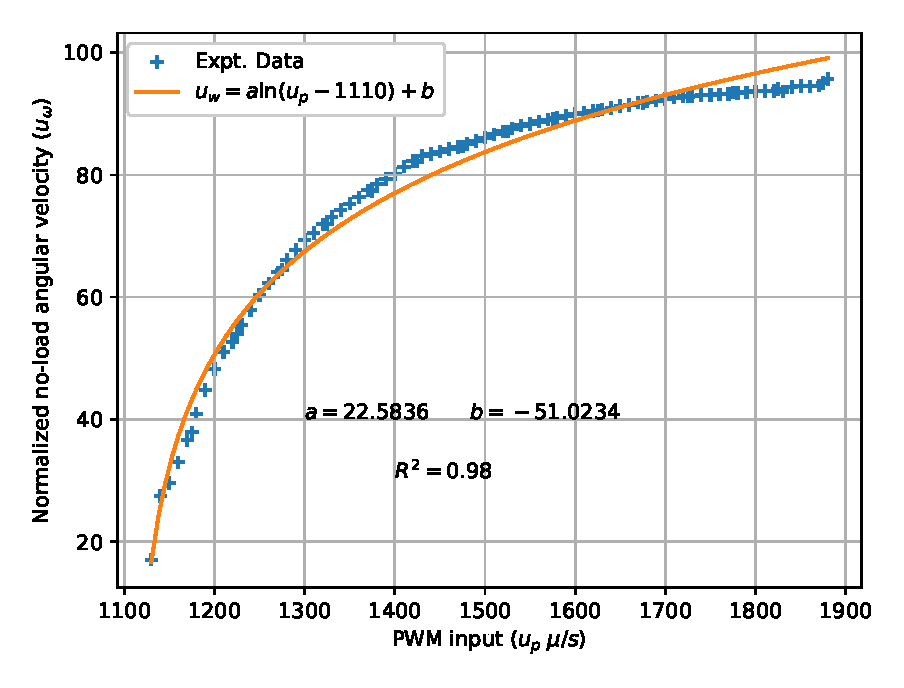
\includegraphics[width = 0.7\textwidth]{./figs/norm_omega/no-load_rpm.eps}
    \caption{Logarithmic fit for $g_w()$}
\end{figure}
Thus,
\begin{align*}
    \boxed{g_w(u_p) = 22 \ln(u_p - 1110)- 47.5 }
\end{align*}
and,
\begin{align*}
    g'_w(u_p) = \frac{22}{u_p - 1110}
\end{align*}


\subsubsection{Static mapping with propeller}
Form eqn.~\ref{eqn:prop} and introducing the normalized input from eqn.~\ref{eqn:norm_in}:
\begin{align*}
    J\dot \omega + (K_rK_v + b_f) \omega + C_D \omega^2 + M_f = u K_r V_{in}
\end{align*}

%===============================================================================
\newpage
\section{BLDC Motor with Propeller Model -- Parameter Estimation}
Intoducing the input definition into the BLDC-motor model with propeller:
\begin{align*}
    J\dot \omega + b_m \omega + C_D \omega^2 + M_f &= u K_r V_{in} = K_r V_{in} g_\omega(u_\omega, \hat V_{in})\\
    \implies  J \dot \omega + b_m \omega + C_D \omega^2 + M_f &= K_r V_{in} \lr{\frac{b_m}{K_r} u_\omega + \frac{\hat V_{in}}{K_r} C_D u_\omega^2 + \frac{M_f}{K_r  \hat V_{in}}}\\
    J \dot \omega + b_m \omega + C_D \omega^2 + M_f \lr{1 - \frac{V_{in}}{\hat V_{in}}} &= V_{in} b_m u_\omega + V_{in} \hat V_{in} C_D u_\omega^2
\end{align*}

\itbf{Note on Voltage:} The battery voltage is assumed to be constant with small variations that can be introduced as uncertainities.
\begin{align*}
    \hat V_{in} &= V_{in} ( 1 + \delta v)
    \implies \frac{V_{in}}{\hat V_{in}} = 1 - \delta v
    \implies \lr{1 - \frac{V_{in}}{\hat V_{in}}} = \delta v
\end{align*}
\begin{equation}
    J \dot \omega + b_m \omega + C_D \omega^2 + M_f \delta v = V_{in} b_m u_\omega + V_{in}^2 (1 + \delta v) C_D u_\omega^2
\end{equation}

%===============================================================================
\subsection{Parametric Identification model for BLDC motor - propeller dyanmcis}
We have:
\begin{equation*}
    J \dot \omega + b_m \omega + C_D \omega^2 + M_f \delta v = V_{in} b_m u_\omega + V_{in}^2 (1 + \delta v) C_D u_\omega^2
\end{equation*}



% Hence, we have the continuous parametric model:
% $$ \dot \omega =
%     \underbrace{\begin{bmatrix}
%     - \omega^2 & - \omega  & -1
% \end{bmatrix}}_{\Phi^T(\omega)}
% \underbrace{\begin{bmatrix}
%     \frac{C_{D}}{J} \\
%     \frac{(K_rK_v + b_f)}{J}  \\
%     M_f \left( 1 - \frac{V_{in}}{\hat V_{in}}\right)
% \end{bmatrix} }_{\pmb \theta}
%     +\left(\frac{(K_rK_v + b_f)}{J} V_{in}\right) u_{\omega}
%  $$

% Let,
% \begin{align*}
%     a_1 = \frac{C_{D}}{J}  \qquad
%     a_2 &= \frac{(K_rK_v + b_f)}{J} \qquad
%     a_3 =   M_f \left( 1 - \frac{V_{in}}{\hat V_{in}}\right)\\
%     \\
%     \pmb \theta = \begin{bmatrix}a_1 & a_2 & a_3 \end{bmatrix}^T &\qquad
%     b = \frac{(K_rK_v + b_f)}{J} V_{in} = a_2 V_{in}
% \end{align*}

% $$\therefore \dot \omega = \Phi^T(\omega) \pmb \theta + b u$$

% \subsubsection{Descritezed Parametric Model}
% Descritizing the above model using euler-method $\left(\dot \omega = \frac{\omega[k] - \omega[k-1]}{h}\right)$, with $h$ as the sampling interval:

% \begin{align*}
%     \frac{\omega[k] - \omega[k-1]}{h} &=
%     \begin{bmatrix} - \omega^2[k-1] & - \omega[k-1]  &  -1 \end{bmatrix}
%     \begin{bmatrix}
%         a_1 \\ a_2 \\ a_3
%     \end{bmatrix}
%     + bu[k-1]\\
%     %===
%     \omega[k] &= h \begin{bmatrix} - \omega^2[k-1] & - \omega[k-1]  & -1 \end{bmatrix}
%     \begin{bmatrix}
%         a_1 \\
%         a_2 - \frac{1}{h} \\
%         a_3 \\
%     \end{bmatrix}
%     + b  h u[k-1]\\
%     %===
%     &= h \begin{bmatrix} - \omega^2[k-1] & -\omega[k-1] & -1 & u[k] \end{bmatrix}
%     \begin{bmatrix}
%         a_1 \\
%         a_2 - \frac{1}{h} \\
%         a_3 \\
%         b
%     \end{bmatrix}
% \end{align*}

% Let,
% \begin{align*}
%     \pmb \theta_h = h
%     \begin{bmatrix}
%         a_1 \\
%         a_2 - \frac{1}{h} \\
%         a_3 \\
%         b
%     \end{bmatrix} =
%     h
%     \begin{bmatrix}
%         \frac{C_{D}}{J} \\
%         \frac{(K_rK_v + b_f)}{J} - \frac{1}{h}  \\
%         M_f \left( 1 - \frac{V_{in}}{\hat V_{in}}\right)\\
%         \frac{(K_rK_v + b_f)}{J} V_{in}
%     \end{bmatrix}
%     \qquad \text{and} \qquad
%     \Phi(\omega[k-1], u[k])^T &=  \begin{bmatrix} - \omega^2[k-1] & -\omega[k-1] & -1 & u[k-1] \end{bmatrix}
% \end{align*}

% hence, we have the parametric model in least-squares form:
% \begin{align*}
%     \omega[k] &= \Phi(\omega[k-1], u[k-1])^T \pmb \theta_h
% \end{align*}

\subsubsection{Input singal (persistance of exitation and frequency limitation)}
\textbf{Note:}
\begin{enumerate}
   \item PE order of a square wave of half-period m is m+1.
   \item PE order of a single sine wave is 2.
\end{enumerate}
%Hence, a sum of sinusoids wave with atleast 3 waves within the frequency of 45 Hz (the limitation is due to the structure) can be used to estimate the parameters and the coefficients of force and torque generated.
%

% ==============================================================================
\subsection{Small Perturbation Model}
We get the linearised model using small perturbtation and neglecting the gain variation $(\delta v)$:
\begin{align*}
    J \delta \dot \omega + b_m \delta \omega + 2 C_D \omega_0 \delta \omega  &= \delta u_\omega \lr{V_{in} b_m + 2V_{in}^2 C_D u_{\omega_0}}\\
    J \delta \dot \omega + (b_m + 2 C_D \omega_0) \delta \omega  &= \delta u_\omega \lr{V_{in} b_m + 2V_{in}^2 C_D u_{\omega_0}}\\
    \text{Laplace Transform:} \qquad \qquad &\\
     \lr{Js + (b_m + 2 C_D \omega_0)} \delta \omega  &= \delta u_\omega \lr{V_{in} b_m + 2V_{in}^2 C_D u_{\omega_0}}
\end{align*}
Thus we have the trannsfer function model:
\begin{align*}
    \frac{\delta \omega(s)}{\delta u_\omega (s)} &= \frac{V_{in} b_m + 2V_{in}^2 C_D u_{\omega_0}}{Js + (b_m + 2 C_D \omega_0)}
\end{align*}
Also, we have the following relationship between the nominal input and outputs from the input-definition:
\begin{align*}
    \omega_0 &= V_{in} u_{\omega_0}\\
    \implies \frac{\delta \omega(s)}{\delta u_\omega (s)} &= \frac{V_{in} \lr{b_m + 2C_D V_{in} u_{\omega_0}}}{Js + (b_m + 2 C_D \omega_0)}
    = \frac{V_{in} \lr{b_m + 2C_D \omega_0}}{Js + (b_m + 2 C_D \omega_0)}\\
    &= \frac{V_{in}}{ \lr{\frac{J}{b_m + 2 C_D \omega_0}} s + 1} \quad \lr{= \frac{K_m}{\tau_m s + 1}}\\
    \implies K_m &= V_{in}\\
    \tau_m &= \frac{J}{b_m + 2 C_D \omega_0}\\
    \implies \omega_m &= \frac{1}{J}\lr{b_m + 2 C_D \omega_0}
\end{align*}

Thus time-constant decreases with the nominal rpm and the static gain is purely a funciton on the battery voltage.

This information will be used for establishing the validity of identified model. Sum-of-Sinusoids input is used around a nominal input for generating the frequency response of the system to identify the model.

In case of using $u_p$ as input:
\begin{align*}
    u_\omega &= a u_p + b\\
    \implies \delta u_\omega &= a \delta u_p\\
    \implies \frac{\delta \omega(s)}{\delta u_p(s)} &= \lr{\frac{1}{a}}\frac{K_m}{\tau_m s + 1}
\end{align*}

Thus this results in variation of the static gain alone.


\subsubsection{Model Parameter Estimation}
The response of the system to Sum-of-Sinusoids signal at $250 \, Hz$ and $50 \mu s$ (PWM) amplitude containing $299$ frequencies in the range $[0.01, 30]\,Hz$ is used for first-order model parameter identification. The nominal inputs and the corresponding $rpm$ is tabulated in Table~\ref{tab::nom_in}. The identified models are validated against the response of a chirp signal with the same frequency range and sampling frequency. The validation results are plotted in Section~\ref{sec::small_perturb_valid}.

\begin{table}[H]
    \centering
    \begin{tabular}{c c c c}
        \hline \hline
        Expt. & $u_{p_0}$ $(\mu s)$& $u_{\omega_0}$ $(rad/(s.V))$ & $\omega_0$ $(rad/s)$ \\ \hline \hline
            1 & 1250      &  22.7035       &  347.1147   \\
            2 & 1300      &  26.1848       &  405.6932   \\
            3 & 1350      &  29.6660       &  460.4567   \\
            4 & 1400      &  33.1472       &  515.9106   \\
            5 & 1450      &  36.6284       &  587.6871   \\
            6 & 1500      &  40.1096       &  646.5961   \\
            7 & 1550      &  43.5908       &  703.7016   \\
            8 & 1600      &  47.0720       &  756.4896   \\
            9 & 1650      &  50.5532       &  806.9497   \\
           10 & 1700      &  54.0344       &  850.6007   \\
           11 & 1750      &  57.5156       &  896.7785   \\
           \hline \hline
    \end{tabular}
    \caption{Nominal Inputs}
    \label{tab::nom_in}
\end{table}


The estimates static-gain and cut-off frequencies are plotted with nominal inputs. The corresopnding parameters relating them to the nominal inputs are estimated using least-squares method.

The $V_{in}$ and $K$ plot demonstrates the validity of their relationship when the $V_{in}$ variation is inclued, i.e.,
\begin{align*}
    K &= V_{in} (1 + \delta v)
\end{align*}

The variation of cut-off frequency with nominal rpm gives the esitmates of propeller moment of inertia and the damping as follows:
\begin{align*}
    J &= 3.2238 \times 10^{-6} \, Kg m^2\\
    b_m &= 0
\end{align*}

\begin{figure}[H]
    \centering
    \begin{minipage}{0.49\textwidth}
        \begin{figure}[H]
            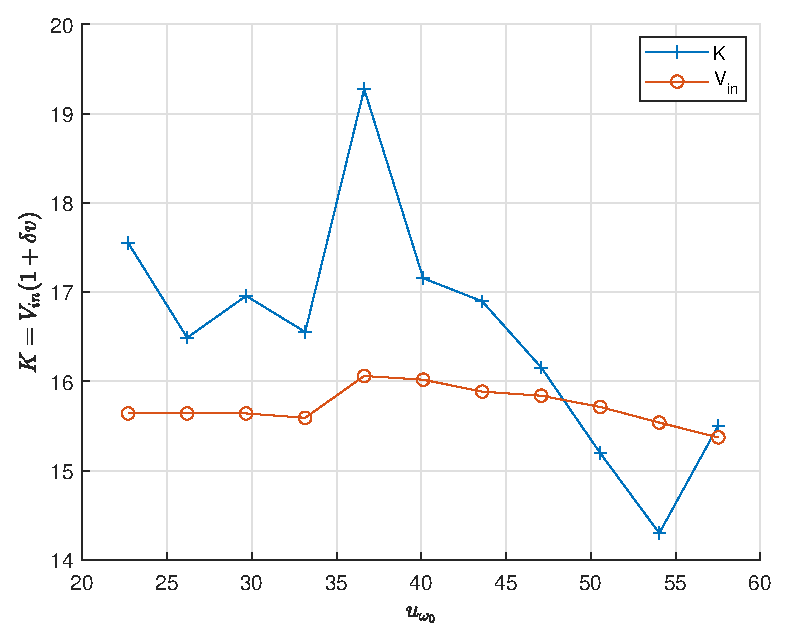
\includegraphics[width = \textwidth]{./figs/small_perturbation/K-Vin.eps}
            \caption{Static gain and Voltage input}
        \end{figure}
    \end{minipage}
    \begin{minipage}{0.49\textwidth}
        \begin{figure}[H]
            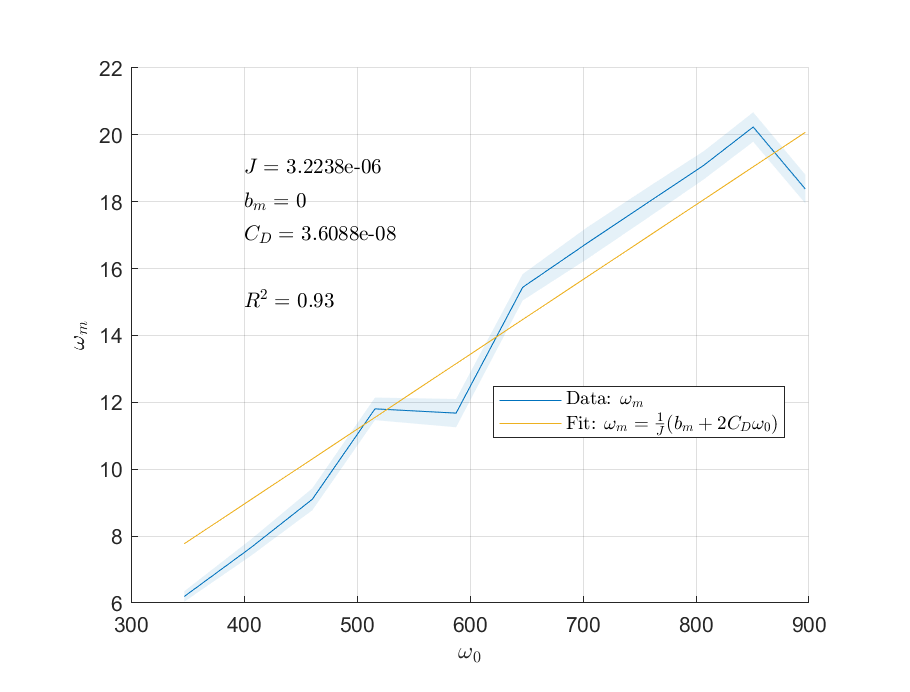
\includegraphics[width = \textwidth]{./figs/small_perturbation/omega_fit.eps}
            \caption{Cut-off frequency}
        \end{figure}
    \end{minipage}
\end{figure}


\begin{table}[H]
    \centering
    \begin{tabular}{c l l}
        \hline \hline
        Parameter & Value & \\ \hline \hline
        $C_T$ & $7.2581 \times 10^{-06}$ & $N/(rad/s)^2$  \\
        $C_D$ & $3.6088 \times 10^{-08}$ & $N.m/(rad/s)^2$ \\
        $b_m$ & $0.0$                    & $N.m/(rad/s)$\\
        $M_f$ & $1.3135 \times 10^{-3}$  & $N.m$\\
        $J$   & $3.2238 \times 10^{-6}$  & $Kg m^2$ \\\hline \hline
    \end{tabular}
    \caption{Summary of parameter estimates from staic and small-perturbation experiments}
\end{table}


%===============================================================================
\newpage
\part{Control}
\section{Control Model and Input}
From parameter estimates (Table~\ref{tab::parm_ests}), it can be seen that the
estimate of total 'damping' factor $( b_m )$ is zero. Thus, the linear term of
the control input in the RHS of eqn.~\ref{eqn::nl_model} can be ignored.
Let $u = u_\omega ^2 $ be the control input to the system for which we are going
to design the feedback controller. Incorporating the above two assumptions into
eqn.~\ref{eqn::nl_model}, we have the control form of the model:
\begin{equation} \label{eqn::control_form}
    J \dot \omega + b_m \omega + C_D \omega^2 + M_f \delta v = V_{in}^2 (1 + \delta v) C_D u
\end{equation}

We have the following bounds on the control input:
\begin{align*}
    u &= u_\omega^2 = \lr{a u_p + b}^2\\
    \implies u_{min} &= \lr{a u_{p_{min}}  + b}^2 = \lr{0.0696 \times 1110 - 64.3266}^2 = 167.1694\\
    \implies u_{max} &= \lr{a u_{p_{max}}  + b}^2 = \lr{0.0696 \times 1890 - 64.3266}^2 = 4518.1789\\
\end{align*}

The goal of feedback control design for the actuator is two-fold:
\begin{enumerate}
\item Compensate for the input-uncertainities, un-modelled disturbances and
model-structure errors.
\item Make the actuator track the response of a second-order transfer function
with no over-shoot of the form:
\begin{align*}
    G_{ref}(s) &= \frac{1}{s^2 + 2 \zeta \omega_{ref} + \omega_{ref}^2}
    && \zeta = \frac{1}{\sqrt{2}} = 0.707
\end{align*}
Such that, $\omega_{ref}$ results in the maximum possible bandwidth in presence
of uncertainties mentioned above.
\end{enumerate}

To this end, two feedback control designs based on Adaptive Robust Control
Theory (ARC) are implemented, and their performances are compared:
\begin{enumerate}
    \item Direct/Indirect Adaptive Robust Controller (DIARC).
    \item ARC design with parameter estimation only for the disturbances(Disturbance ARC).
    \item Feedback linearization.
\end{enumerate}

%===============================================================================
\subsection{Parametric model and parameter bounds for ARC design}

The parameter bounds are obtained from the variance of estimates and the
maximum value of $\delta v$. For the current design $\pm 2\sigma$ bounds are
used for each of the $\theta$'s. From experimental observations, the maximum
supply voltage is about $16\, V$ and minimum supply voltage is close to $15\,
V$. The average would be in the middle ($15.5\, V$). The physics dictates that
all the physical parameters have a non-negative value. Also, the minimum value
of $J$ is assumed to be $1/10$ of its nominal value instead of zero. This is to
ensure that the inertia estimate would never be zero and with-in the reasonable
limits. The following table gives the minimum, maximum and nominal values of the parameters:

\begin{table}[H]
    \centering
    \begin{tabular}{r l r r r}
        \hline \hline
        Parameter & Units &Nominal & Minimum & Maximum \\ \hline \hline
        $C_T$                   &
        $N/(rad/s)^2$           &
        $7.2581e-6$             &
        $7.1690e-6$             &
        $7.3471e-6$
        \\
        $C_D$                   &
        $N.m/(rad/s)^2$         &
        $3.6088e-8$             &
        $3.3295e-8$             &
        $3.8881e-8$

        \\
        $b_m$                    &
        $N.m/(rad/s)$            &
        $0$                      &
        $0$                      &
        $9.2006e-6$
        \\
        $M_f$                    &
        $N.m$                    &
        $1.3135e{-3}$            &
        $0$                      &
        $0.0104$
        \\
        $J$                      &
        $Kg.m^2$                 &
        $3.2238e{-6}$            &
        $3.2238e{-7}$            &
        $1.7234e-5$
        \\
        $V_{in}$                 &
        $V$                      &
        $15.5$                   &
        $15$                     &
        $16$
        \\
        $\delta v$               &
                                 &
        $0$                      &
        $-0.2$                   &
        $0.2$
        \\
        \hline \hline
    \end{tabular}
    \caption{Summary of parameter bounds}
    \label{tab::parm_bounds}
\end{table}

\subsubsection{Parametric Model}
It can be noted that the variance of $\hat J$ is substantial as compared to its
actual value. This would propagate into the all the parameters if it is divided
on all sides. Instead, we normalize all the coefficients with the controller
gain to minimize the propagation of variance to the parameters. Thus,
eqn.~\ref{eqn::control_form} becomes:

\begin{align*}
    \lr{\frac{J}{V_{in}^2 C_D}} \dot \omega + \lr{\frac{b_m}{V_{in}^2 C_D}} \omega + \lr{\frac{1}{V_{in}^2}} \omega^2  &= u + \delta v \lr{u - \frac{M_f}{V_{in}^2 C_D}}\\
    %===
    \text{Let, } \qquad &\\
    \theta_1 = \lr{\frac{J}{V_{in}^2 C_D}} \qquad
    \theta_2 &= \lr{\frac{b_m}{V_{in}^2 C_D}}\qquad
    \theta_3 = \lr{\frac{1}{V_{in}^2}}\\
    d(t) &= \delta v \lr{u - \frac{M_f}{V_{in}^2 C_D}}\\
    %===
    \implies \theta_1 \dot \omega + \theta_2 \omega + \theta_3 \omega^2 &= u + d(t)
\end{align*}
\begin{equation}\label{eqn::almst_ctrl_mdl}
    \theta_1 \dot \omega = u - \theta_2 \omega - \theta_3 \omega^2 + d(t)
\end{equation}

Let, $\omega_d(t)$ be the desired trajectory that the system needs to track
(output of $G_{ref}(s)$). Thus, the tracking error:
\begin{align*}
    s &= \omega - \omega_d \quad \implies \dot s = \dot \omega - \dot \omega_d
\end{align*}
Dividing the disturbance into high-frequency component and a slowly varying
component, let, $$d(t) = d_0 + \Delta(t)$$
Thus, subtracting $\theta_1 \omega_d$ on both sides of eqn.~\ref{eqn::almst_ctrl_mdl}.
\begin{align*}
    \theta_1 (\dot \omega - \dot \omega_d) &= u - \theta_1 \omega_d - \theta_2 \omega - \theta_3 \omega^2 + d_0 + \Delta(t)\\
    \text{Let,} \qquad\\
    \pmb \theta &= \bm{\theta_1 & \theta_2 & \theta_3 & d_0}^T\\
    \pmb \phi &= \bm{-\omega_d & -\omega & - \omega^2 & 1}^T\\
\end{align*}
Thus we have the model for tracking error dynamics:
\begin{equation}\label{eqn::error_dyn}
    \theta_1 \dot s = u + \pmb \phi^T \pmb \theta + \Delta(t)
\end{equation}


\subsubsection{Parameter Bounds}
The parameter bounds for eqn.~\ref{eqn::error_dyn} are obtained from the
parameter bounds of estimated parameters. Also,
\begin{align*}
    \abs{d(t)} &\leq d_M \implies \abs{d_0} \leq d_M \text{  and  } \abs{\Delta} \leq 2d_M = \Delta_M\\
    \text{From Table~\ref{tab::parm_bounds}} \qquad &\\
    d_M &= \delta v_{max} \lr{u_{max} - \frac{M_{f_{min}}}{V_{in_{max}}^2 C_{D_{max}}}} \approx 900
\end{align*}
Similarly, we have
\begin{table}[H]
    \centering
    \begin{tabular}{r l r r r}
        \hline \hline
        Parameter & Equation & Nominal & Minimum & Maximum\\ \hline \hline
        $\theta_1$ &
        $= \lr{\frac{J}{V_{in}^2 C_D}}$ &
        $3.7183e-1$ &
        $3.2388e-2$ &
        $2.3005$
        \\
        $\theta_2$ &
        $= \lr{\frac{b_m}{V_{in}^2 C_D}}$ &
        $0$ &
        $0$ &
        $1.0794$
        \\
        $\theta_3$ &
        $= \lr{\frac{1}{V_{in}^2}}$ &
        $4.1623e-3$ &
        $3.9062e-3$ &
        $4.4444e-3$
        \\
        \hline \hline
    \end{tabular}
    \caption{Parameter Bounds}
    \label{tab::parm_lims}
\end{table}

%===============================================================================
\newpage
\section{Characterizing the Effects of Modelling Uncertainities and Assumptions}
The modelling uncertainities due to the uncertainities in the input definition
and the parameter estimates affect the tracking performance of the controller.
The primary sources of the uncertainities are as follows:
\begin{enumerate}
    \item Uncertainities due to the input definition.
    \begin{enumerate}
        \item Uncertainities caused by neglecting the linear term in the input based on
        the assumptions $b_m = 0 \implies V_{in} b_m u_\omega = 0$.
        \item Effects of non-zero and slowly varying $\delta v$.
    \end{enumerate}

    \item Uncertainities in the model parameter estimates.
\end{enumerate}

The effects of the uncertainities are determined by the relative error in the
prediction from the nominal model and the model with only that particular uncertainity.

\subsection{Effects of non-zero $b_m$}
From the simulink model the uncertainity in $b_m$ does'nt effect the prediction
error significantly. A $3 \sigma$ variation in $b_m$ produced less than $1\%$
relative error in the prediction. Thus, $b_m$ can be completely neglected out of
the non-linear model without significant prediction errors.

\begin{figure}[H]
\begin{minipage}{0.49\textwidth}
    \begin{figure}[H]
        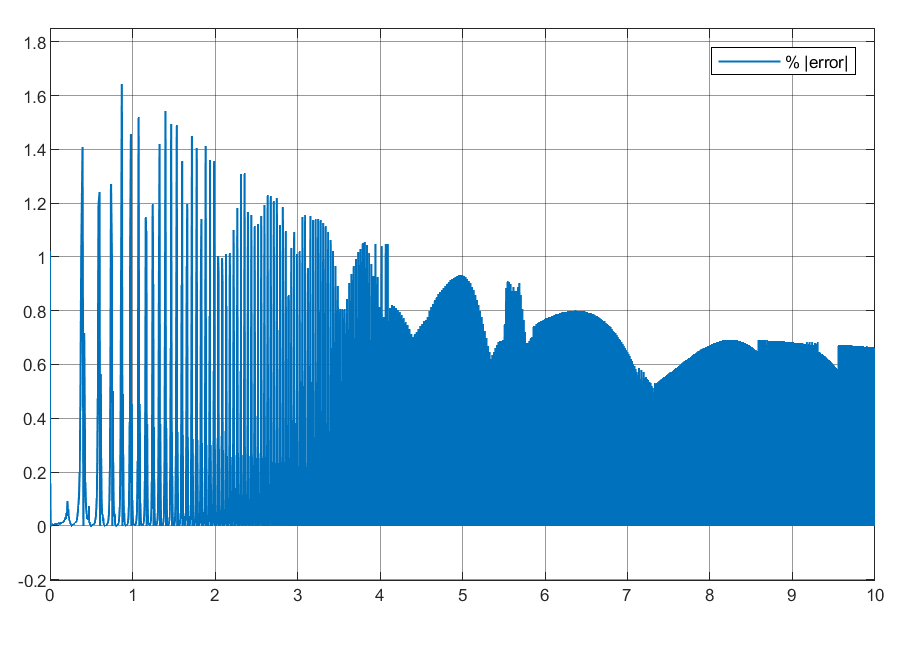
\includegraphics[width = \textwidth]{figs/par_var/3_sig_bm.eps}
        \caption{$\%$ error for $3 \sigma$ variation in $b_m$}
    \end{figure}
\end{minipage}
\begin{minipage}{0.49\textwidth}
    \begin{figure}[H]
        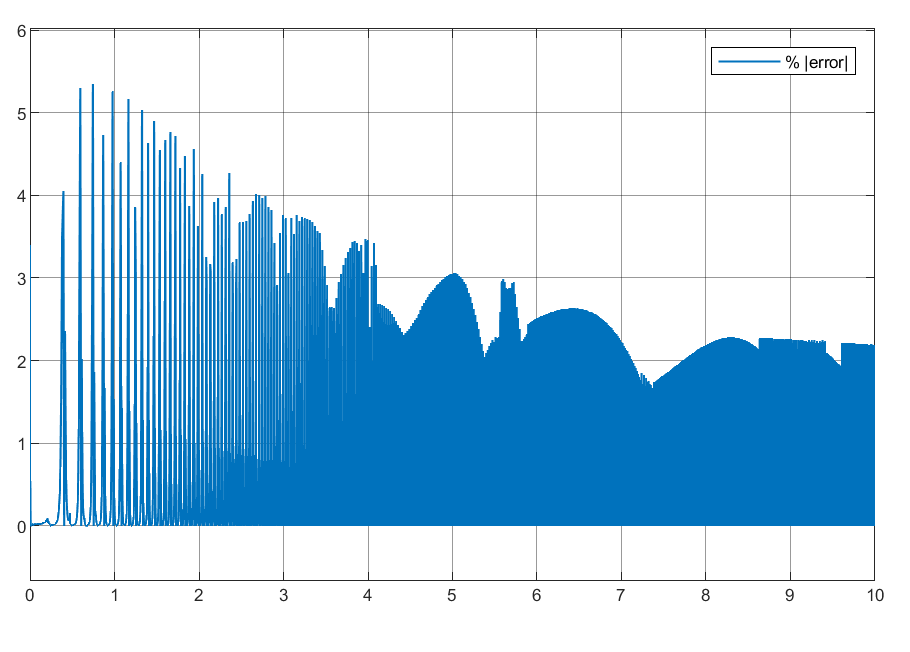
\includegraphics[width = \textwidth]{figs/par_var/10_sig_bm.eps}
        \caption{$\%$ error for $10 \sigma$ variation in $b_m$}
    \end{figure}
\end{minipage}
\end{figure}

\subsection{Effects of non-zero $\delta v$}
$\delta v$ significantly effects the prediction error as it is effectivly
changes the input-gain and also introduces un-compensated friction into the
system.
\begin{figure}[H]
\begin{minipage}{0.49\textwidth}
    \begin{figure}[H]
        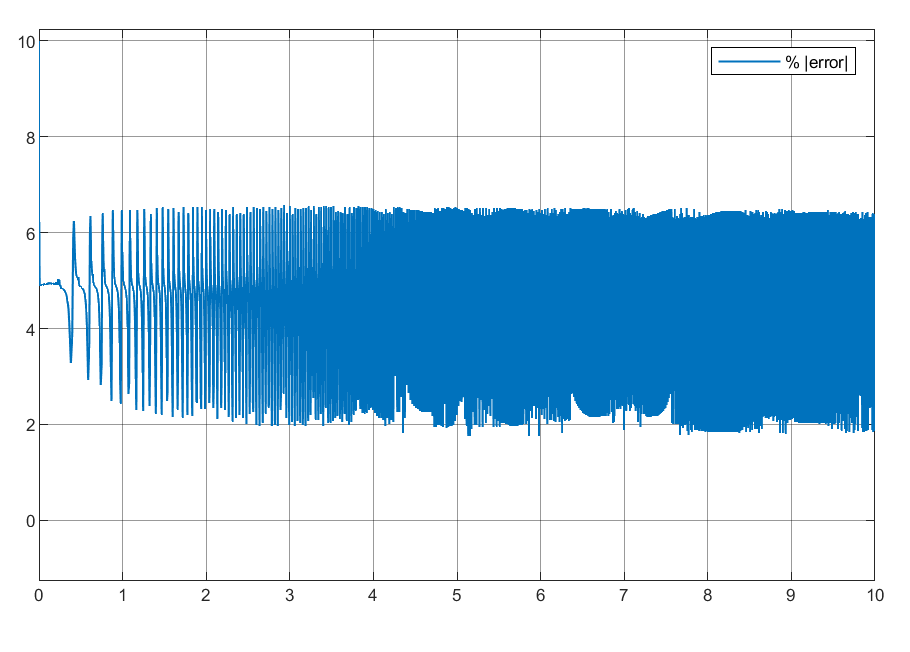
\includegraphics[width = \textwidth]{figs/par_var/1_del_v.eps}
        \caption{$\%$ error $\delta v = 0.1$}
    \end{figure}
\end{minipage}
\begin{minipage}{0.49\textwidth}
    \begin{figure}[H]
        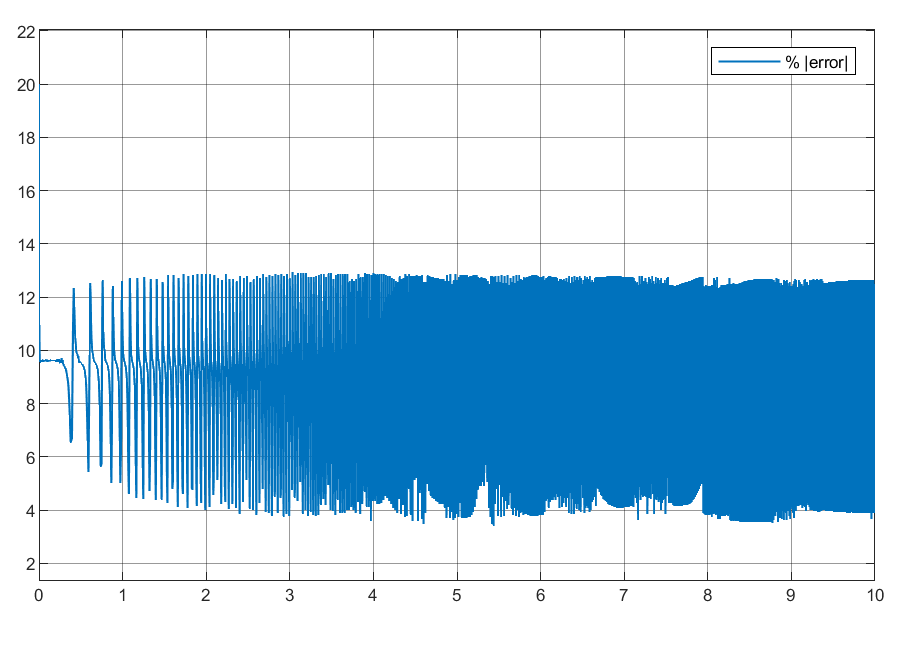
\includegraphics[width = \textwidth]{figs/par_var/2_del_v.eps}
        \caption{$\%$ error for $\delta v = 0.2$}
    \end{figure}
\end{minipage}
\end{figure}


\subsection{Effects of model-parameter estimation errors}
The parameter $J, C_D$ effect the prediction errors to the same order of
magnitude to their estimation errors. The figures bellow show the effect of
$10\%$ estimation errors in their parameters.

\begin{figure}[H]
\begin{minipage}{0.49\textwidth}
    \begin{figure}[H]
        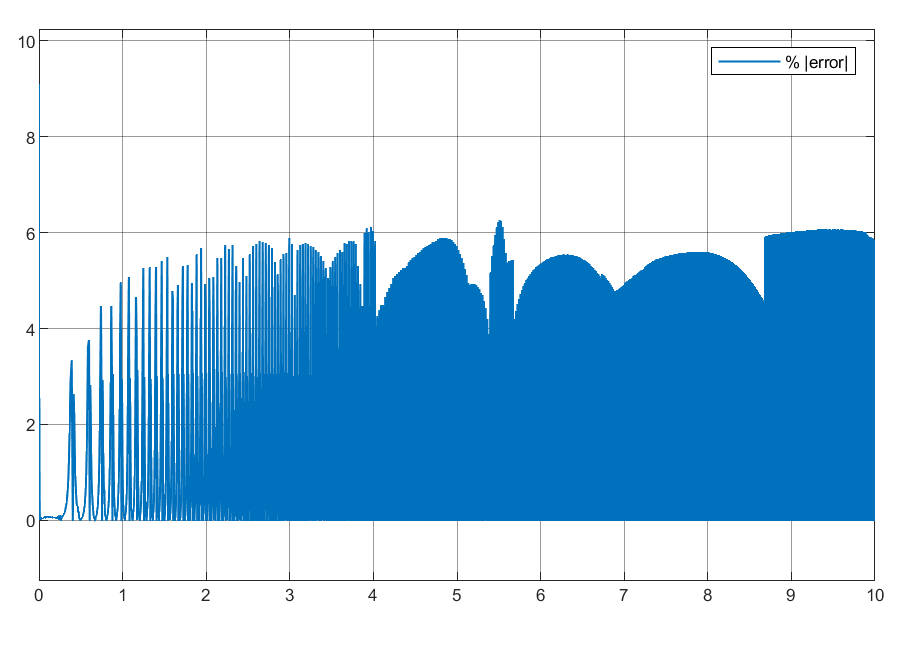
\includegraphics[width = \textwidth]{figs/par_var/j.eps}
        \caption{$\%$ error for $10\%$ error in J}
    \end{figure}
\end{minipage}
\begin{minipage}{0.49\textwidth}
    \begin{figure}[H]
        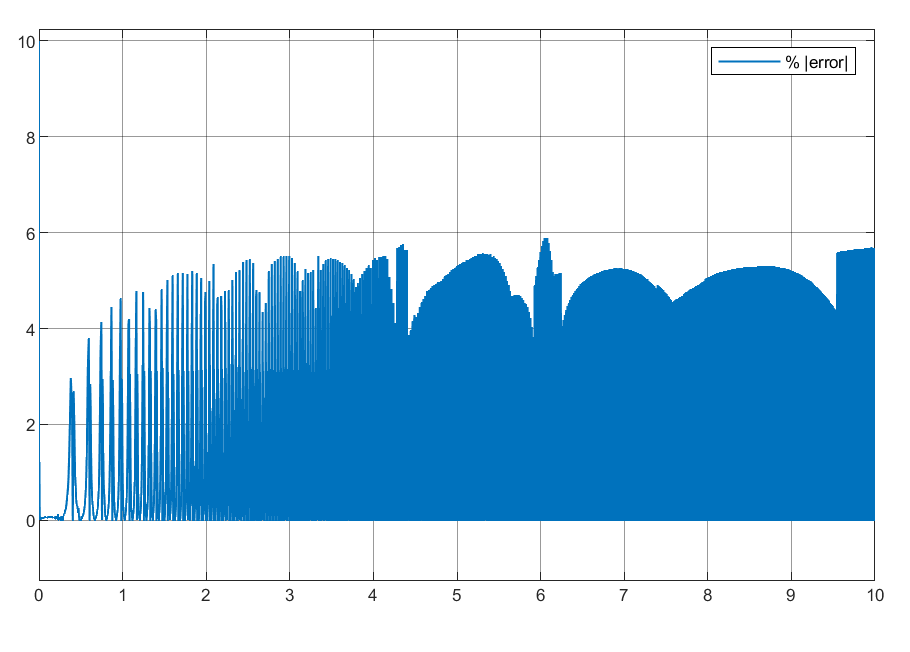
\includegraphics[width = \textwidth]{figs/par_var/c_d.eps}
        \caption{$\%$ error for $10\%$ error in $C_D$}
    \end{figure}
\end{minipage}
\end{figure}

The effect of $M_f$ is indirectly effects $\delta v$. These errors have to be
lumped together for estimation.
    \begin{figure}[H]
        \centering
        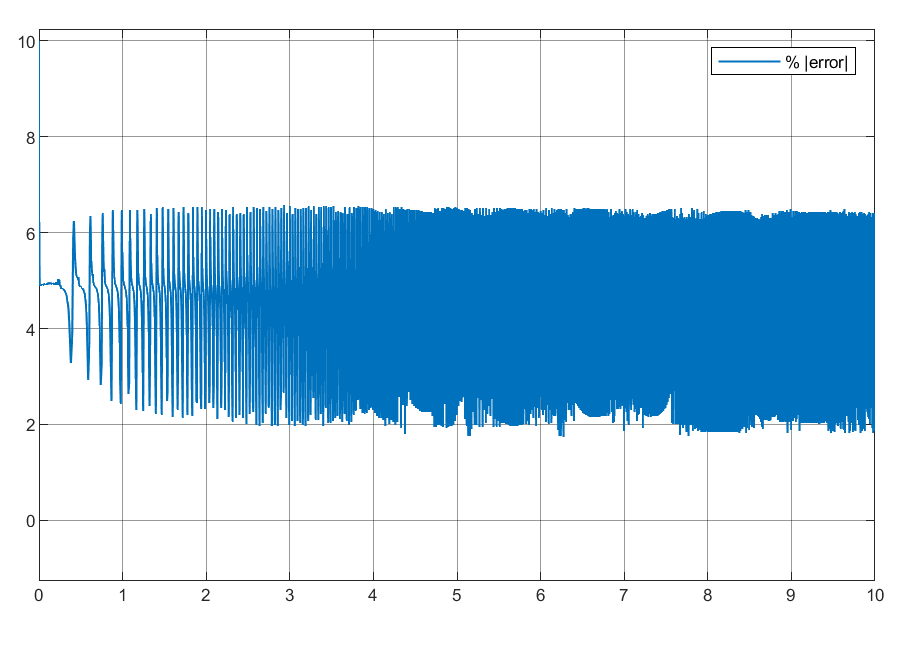
\includegraphics[width = 0.49\textwidth]{figs/par_var/m_f.eps}
        \caption{$\%$ error for $10\%$ error in $M_f$ with $\delta v=0.1$}
    \end{figure}


\subsection{Conclusion}
Thus from above analysis, we conclude following:

\begin{enumerate}
\item The model parameters that significantly effect the tracking performance
are (in the order of their infulunce): $1) \delta v, \, 2) M_f, \, 3)J, \, 4) C_D$
\item The linear damping factor of the motor $b_m$ doesn't significantly effect
the tracking performance of the system with-in it's estimation error. Hence, it can be removed from model simplifiying the model structure and the number of
model parameters to be estimated. Further, this analysis justifies the
assummption used to arrive at the control form \ref{eqn::control_form}. Thus, eqn. (\ref{eqn::control_form}) becomes:
\end{enumerate}

\begin{equation}\label{eqn::no_bm_ctrl_form}
    J \dot \omega + C_D \omega^2 + M_f \delta v = V_{in}^2 (1 + \delta v) C_D u_\omega^2
\end{equation}

%===============================================================================
\newpage
\section{Conclusion}
\newpage
\section{Appendix}
\subsection{Linearized Model Validation \label{sec::small_perturb_valid}}

\subsubsection{Frequency Domain Validation}
%===============================================================================
\begin{figure}[H]
    \begin{minipage}{0.32\textwidth}
       \begin{figure}[H]
            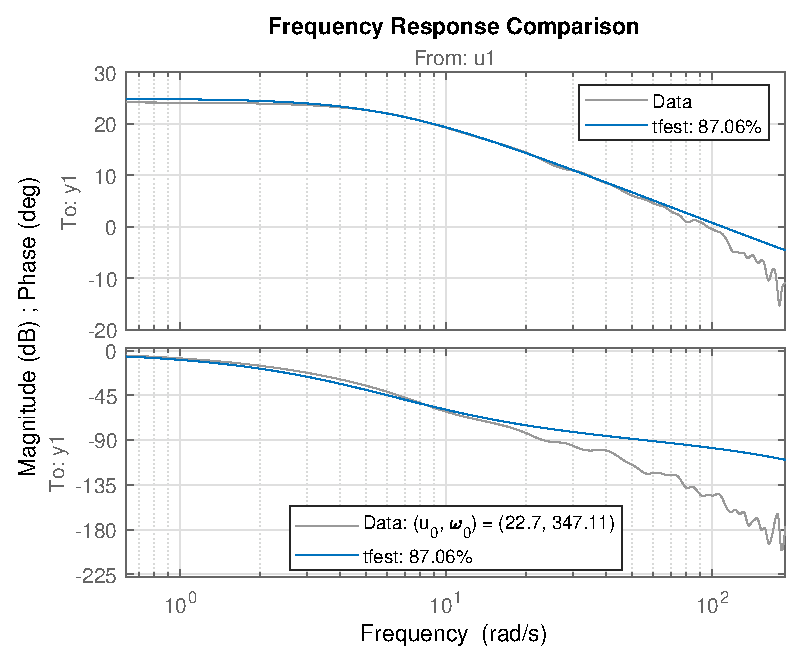
\includegraphics[width = \textwidth]{./figs/small_perturbation/freq_Compare_1250.eps}
       \end{figure}
    \end{minipage}
    \begin{minipage}{0.32\textwidth}
       \begin{figure}[H]
            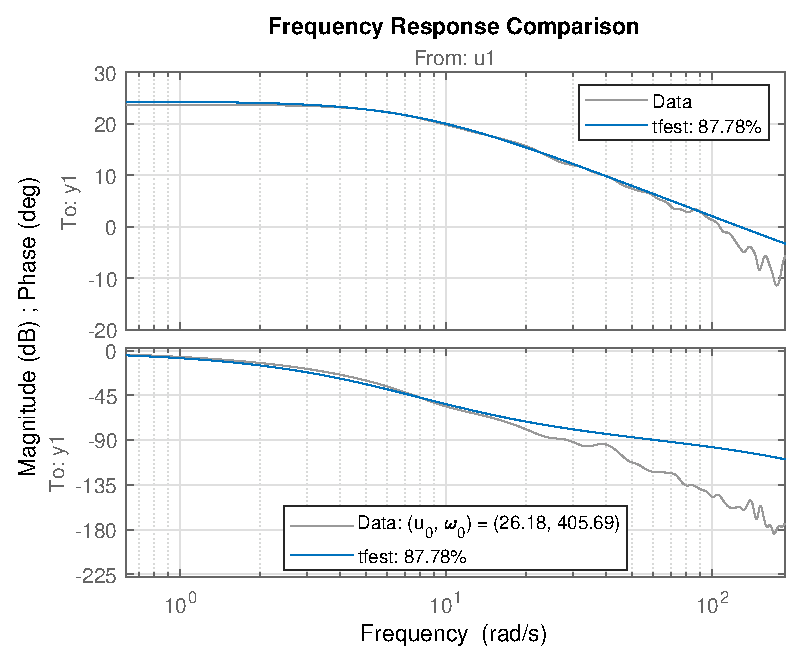
\includegraphics[width = \textwidth]{./figs/small_perturbation/freq_Compare_1300.eps}
       \end{figure}
    \end{minipage}
    \begin{minipage}{0.32\textwidth}
       \begin{figure}[H]
            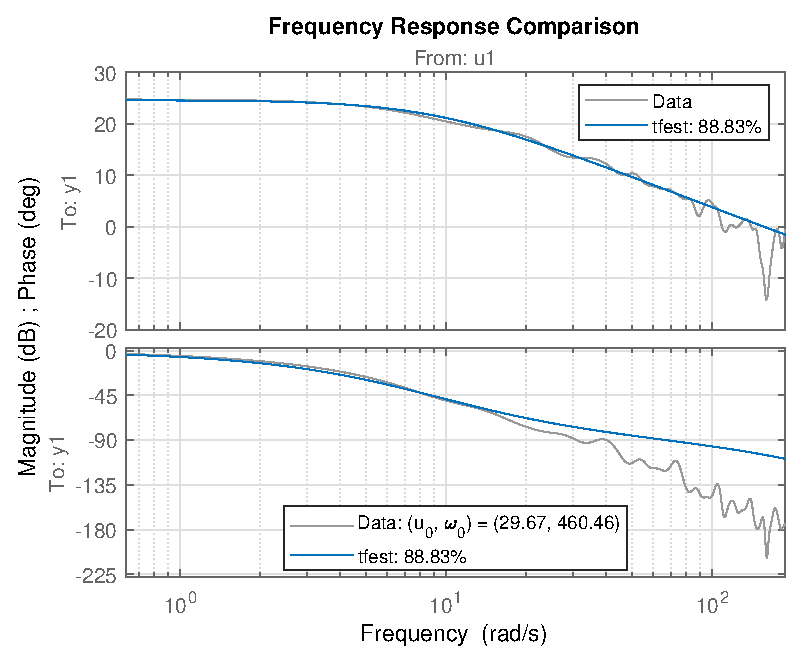
\includegraphics[width = \textwidth]{./figs/small_perturbation/freq_Compare_1350.eps}
       \end{figure}
    \end{minipage}
\end{figure}
%-------------------------------------------------------------------------------
\begin{figure}[H]
    \begin{minipage}{0.32\textwidth}
       \begin{figure}[H]
            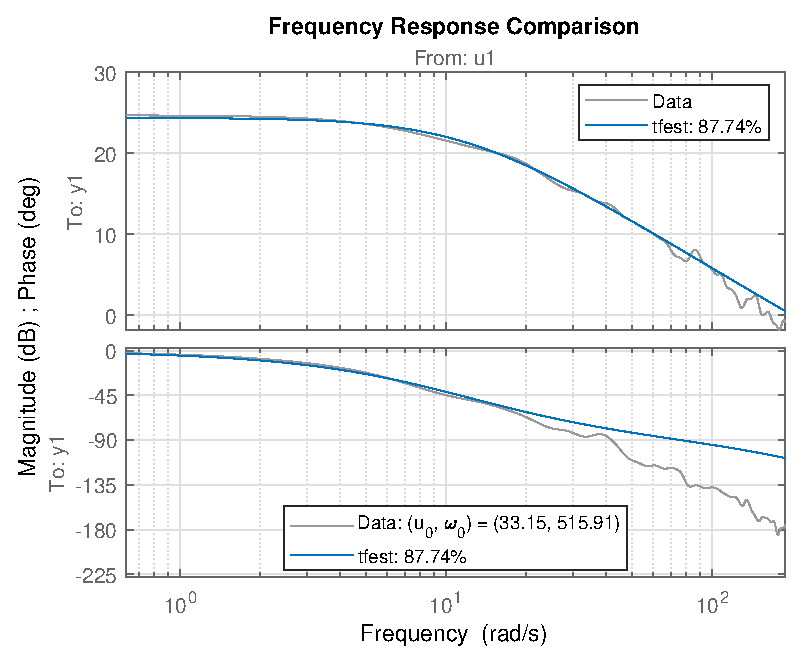
\includegraphics[width = \textwidth]{./figs/small_perturbation/freq_Compare_1400.eps}
       \end{figure}
    \end{minipage}
    \begin{minipage}{0.32\textwidth}
       \begin{figure}[H]
            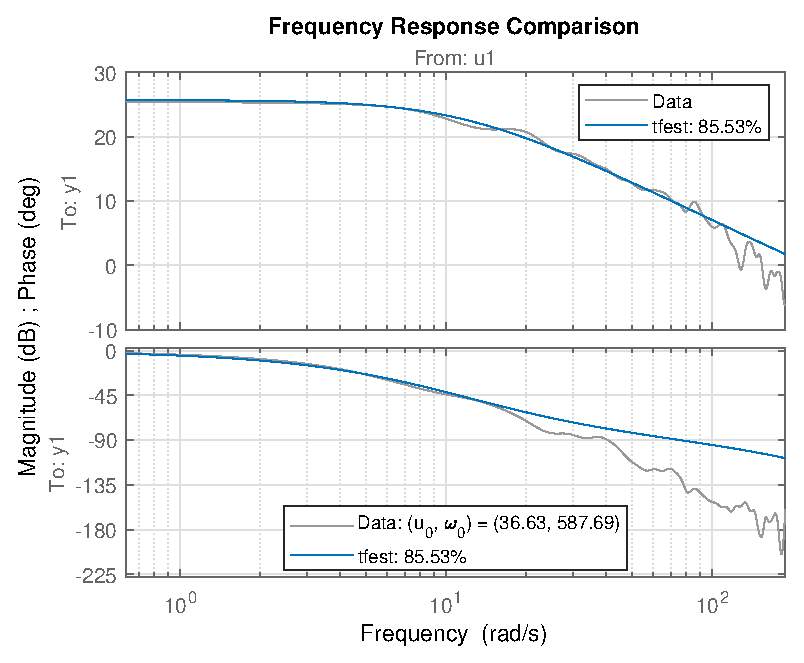
\includegraphics[width = \textwidth]{./figs/small_perturbation/freq_Compare_1450.eps}
       \end{figure}
    \end{minipage}
    \begin{minipage}{0.32\textwidth}
       \begin{figure}[H]
            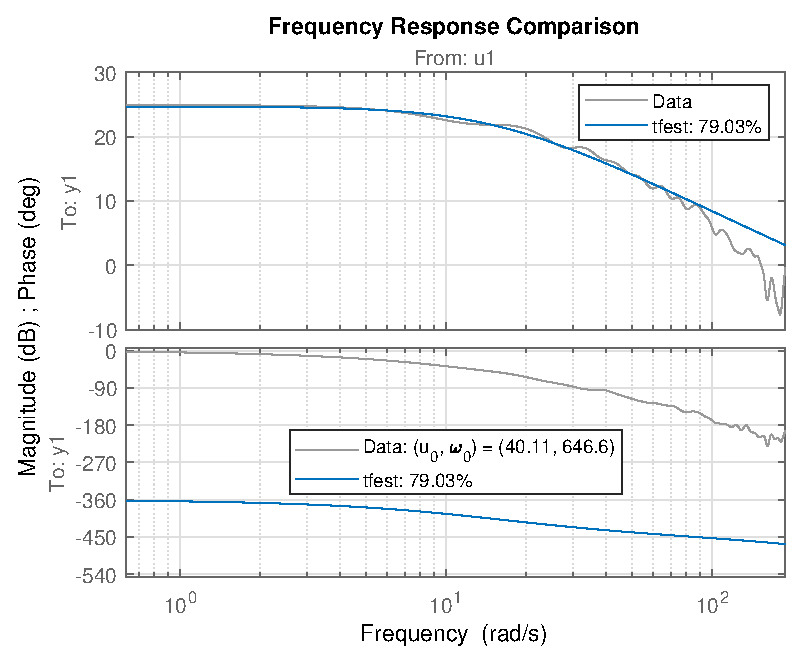
\includegraphics[width = \textwidth]{./figs/small_perturbation/freq_Compare_1500.eps}
       \end{figure}
    \end{minipage}
\end{figure}
%-------------------------------------------------------------------------------
\begin{figure}[H]
    \begin{minipage}{0.32\textwidth}
       \begin{figure}[H]
            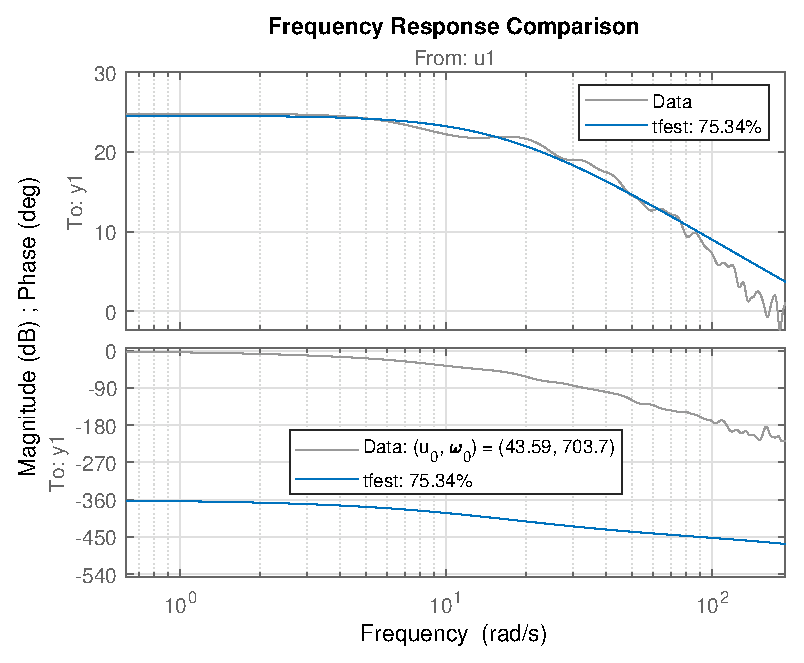
\includegraphics[width = \textwidth]{./figs/small_perturbation/freq_Compare_1550.eps}
       \end{figure}
    \end{minipage}
    \begin{minipage}{0.32\textwidth}
       \begin{figure}[H]
            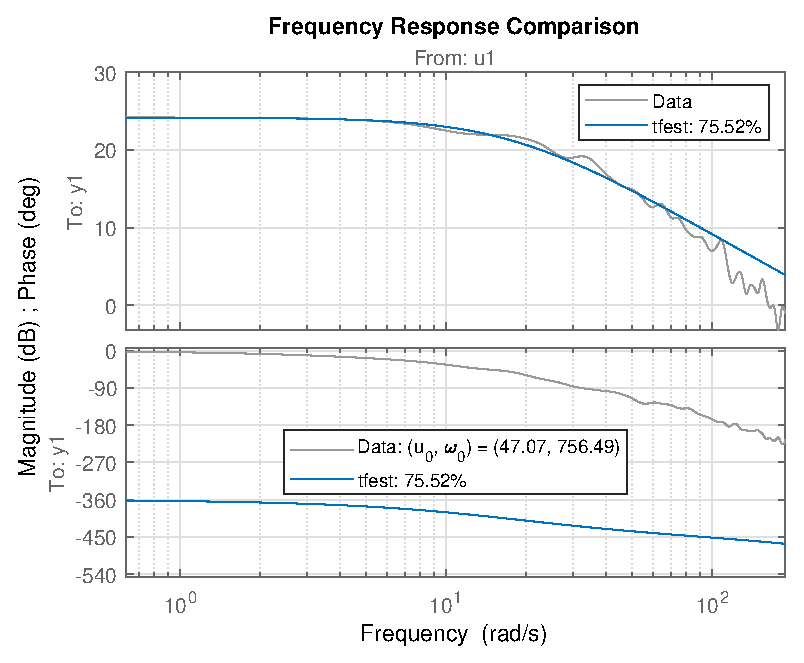
\includegraphics[width = \textwidth]{./figs/small_perturbation/freq_Compare_1600.eps}
       \end{figure}
    \end{minipage}
    \begin{minipage}{0.32\textwidth}
       \begin{figure}[H]
            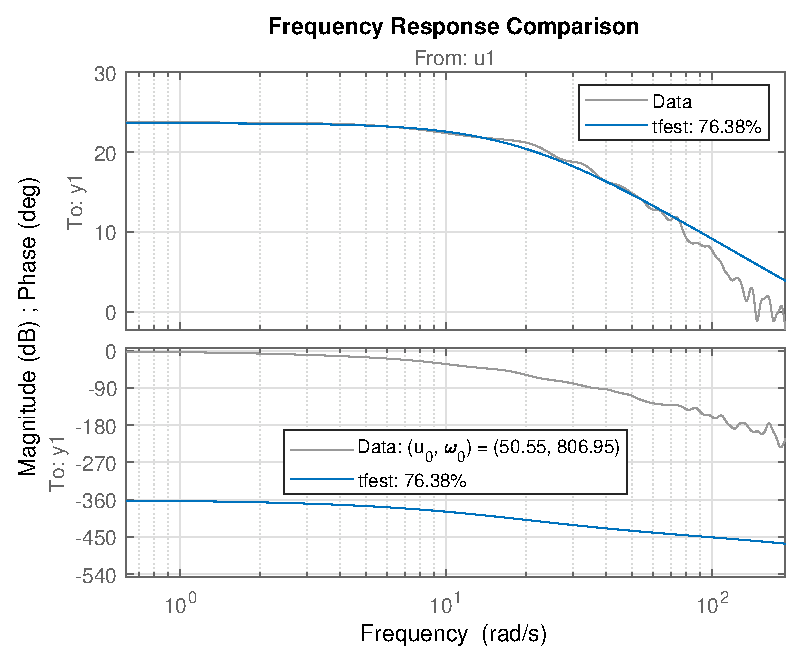
\includegraphics[width = \textwidth]{./figs/small_perturbation/freq_Compare_1650.eps}
       \end{figure}
    \end{minipage}
\end{figure}
%-------------------------------------------------------------------------------
\begin{figure}[H]
    \centering
    \begin{minipage}{0.32\textwidth}
       \begin{figure}[H]
            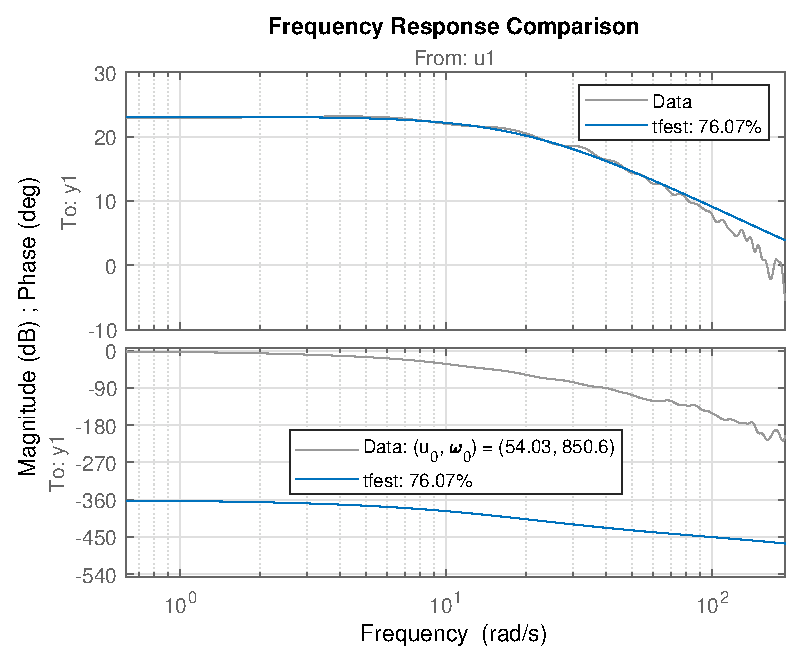
\includegraphics[width = \textwidth]{./figs/small_perturbation/freq_Compare_1700.eps}
       \end{figure}
    \end{minipage}
    \begin{minipage}{0.32\textwidth}
       \begin{figure}[H]
            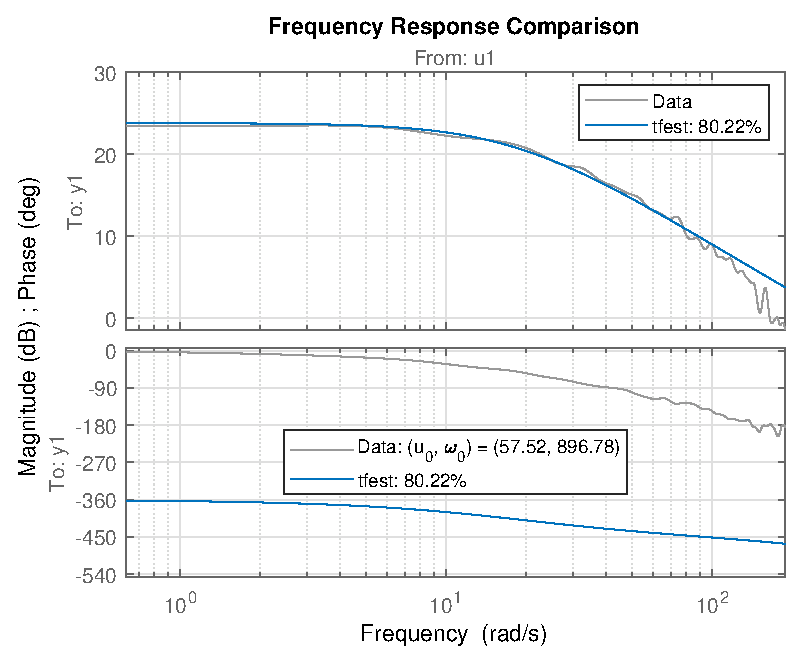
\includegraphics[width = \textwidth]{./figs/small_perturbation/freq_Compare_1750.eps}
       \end{figure}
    \end{minipage}
\end{figure}


\subsubsection{Time Domain Validation}
%===============================================================================
\begin{figure}[H]
    \begin{minipage}{0.32\textwidth}
       \begin{figure}[H]
            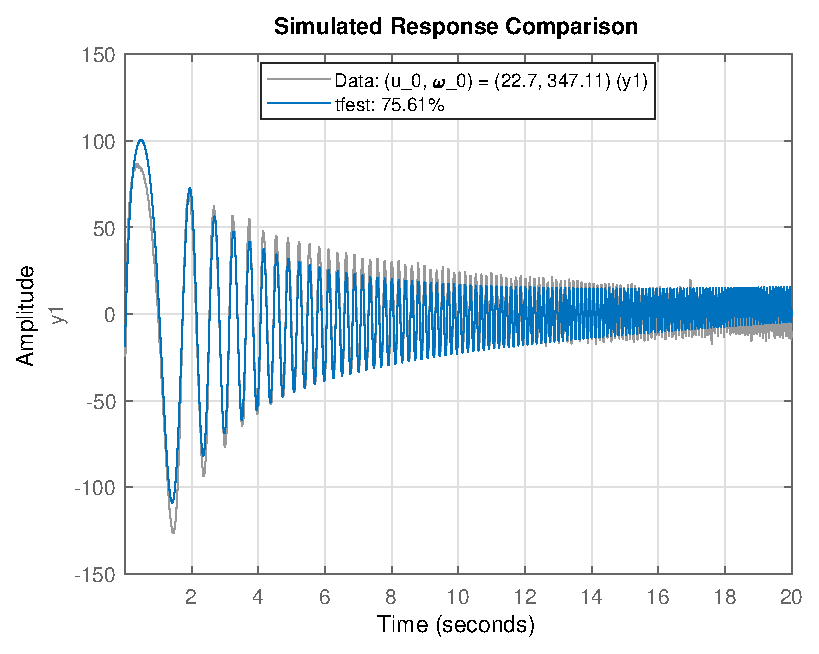
\includegraphics[width = \textwidth]{./figs/small_perturbation/time_Compare_1250.eps}
       \end{figure}
    \end{minipage}
    \begin{minipage}{0.32\textwidth}
       \begin{figure}[H]
            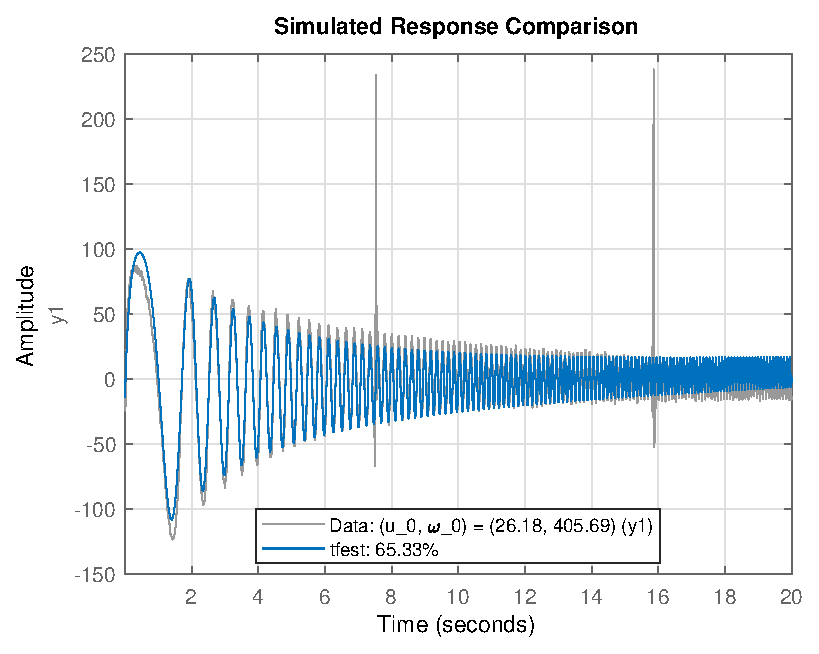
\includegraphics[width = \textwidth]{./figs/small_perturbation/time_Compare_1300.eps}
       \end{figure}
    \end{minipage}
    \begin{minipage}{0.32\textwidth}
       \begin{figure}[H]
            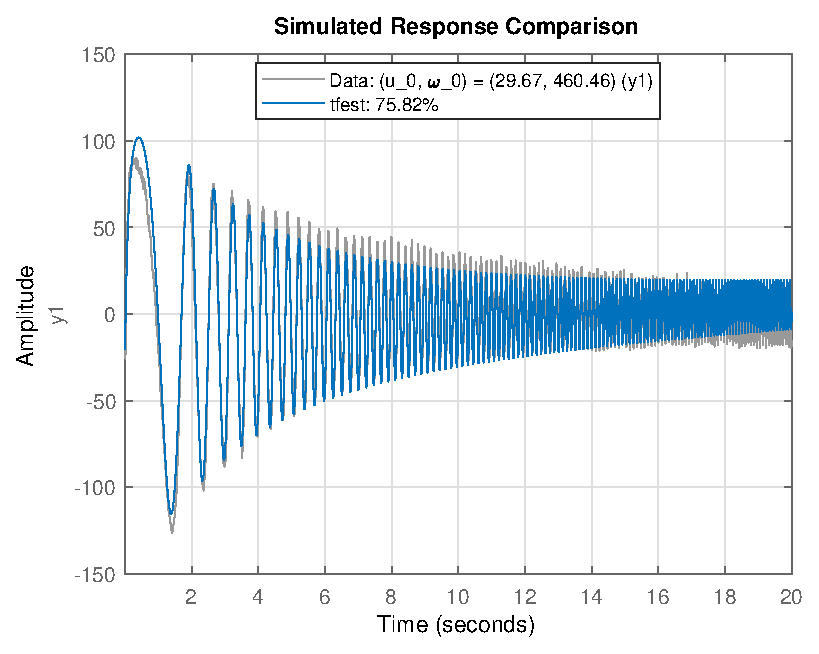
\includegraphics[width = \textwidth]{./figs/small_perturbation/time_Compare_1350.eps}
       \end{figure}
    \end{minipage}
\end{figure}
%-------------------------------------------------------------------------------
\begin{figure}[H]
    \begin{minipage}{0.32\textwidth}
       \begin{figure}[H]
            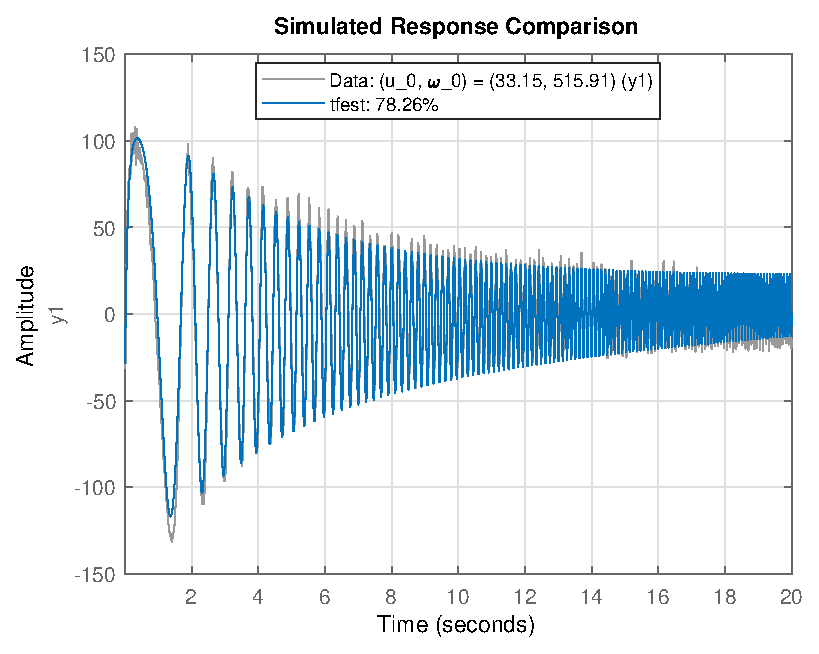
\includegraphics[width = \textwidth]{./figs/small_perturbation/time_Compare_1400.eps}
       \end{figure}
    \end{minipage}
    \begin{minipage}{0.32\textwidth}
       \begin{figure}[H]
            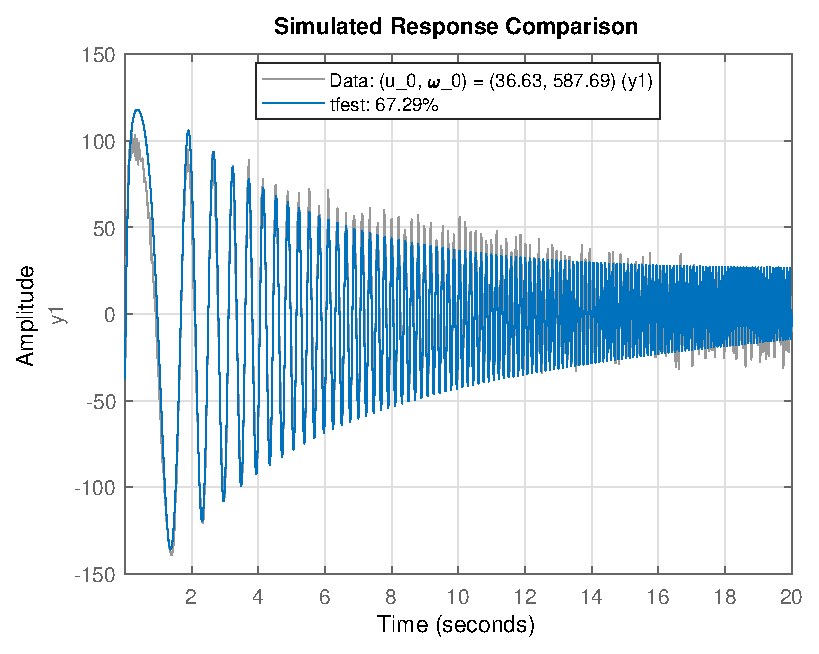
\includegraphics[width = \textwidth]{./figs/small_perturbation/time_Compare_1450.eps}
       \end{figure}
    \end{minipage}
    \begin{minipage}{0.32\textwidth}
       \begin{figure}[H]
            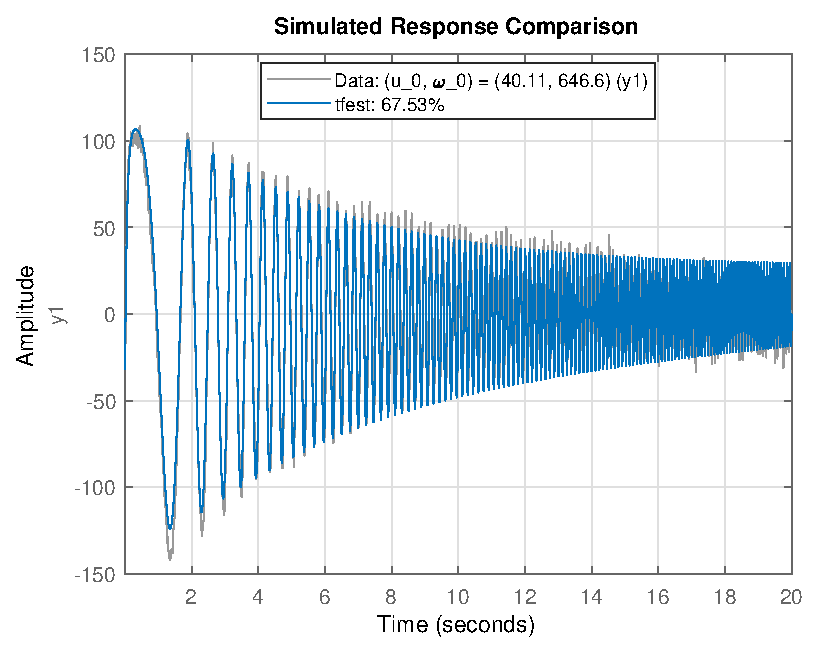
\includegraphics[width = \textwidth]{./figs/small_perturbation/time_Compare_1500.eps}
       \end{figure}
    \end{minipage}
\end{figure}
%-------------------------------------------------------------------------------
\begin{figure}[H]
    \begin{minipage}{0.32\textwidth}
       \begin{figure}[H]
            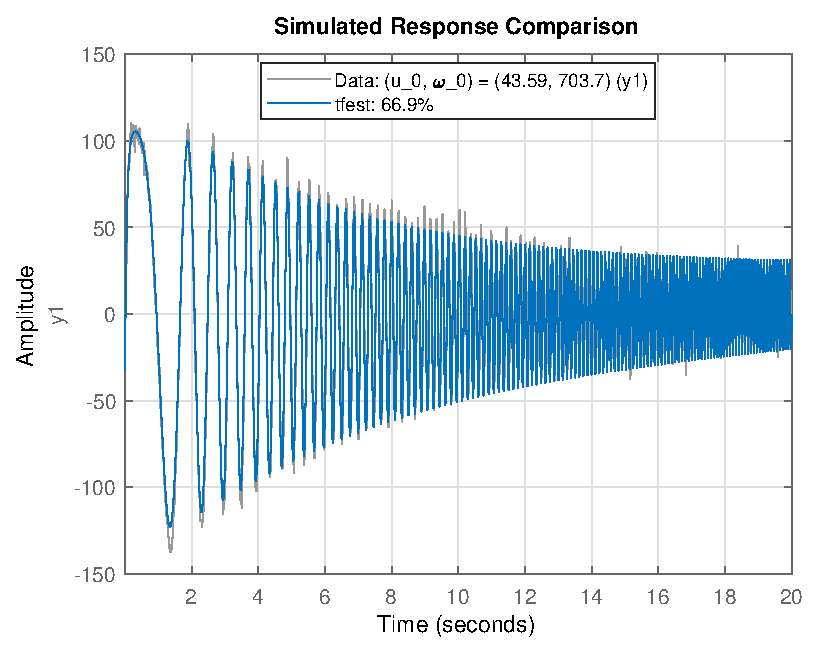
\includegraphics[width = \textwidth]{./figs/small_perturbation/time_Compare_1550.eps}
       \end{figure}
    \end{minipage}
    \begin{minipage}{0.32\textwidth}
       \begin{figure}[H]
            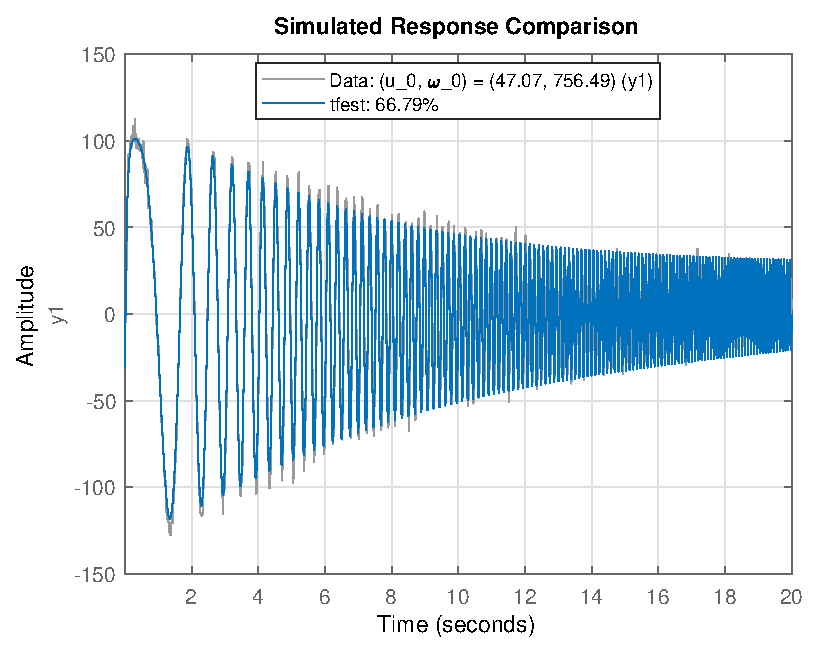
\includegraphics[width = \textwidth]{./figs/small_perturbation/time_Compare_1600.eps}
       \end{figure}
    \end{minipage}
    \begin{minipage}{0.32\textwidth}
       \begin{figure}[H]
            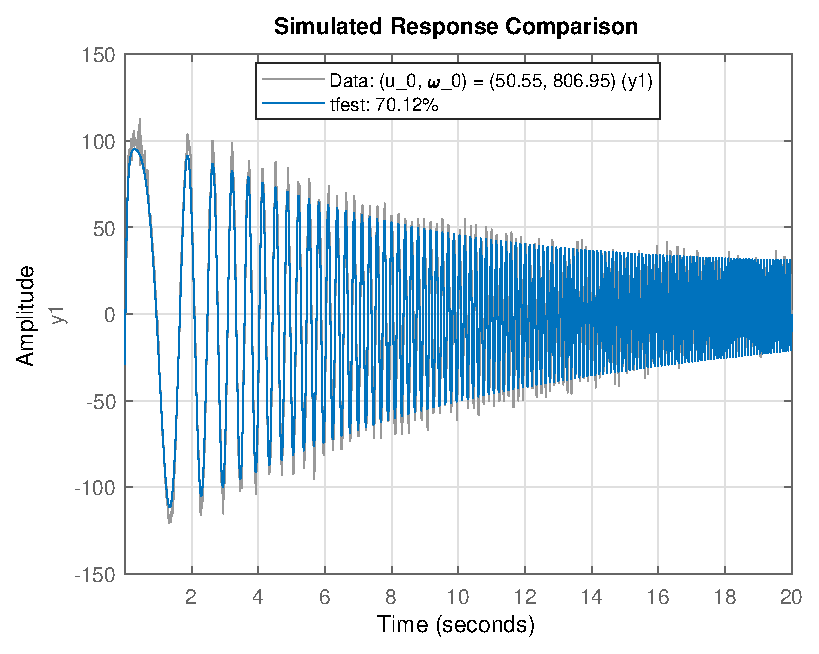
\includegraphics[width = \textwidth]{./figs/small_perturbation/time_Compare_1650.eps}
       \end{figure}
    \end{minipage}
\end{figure}
%-------------------------------------------------------------------------------
\begin{figure}[H]
    \centering
    \begin{minipage}{0.32\textwidth}
       \begin{figure}[H]
            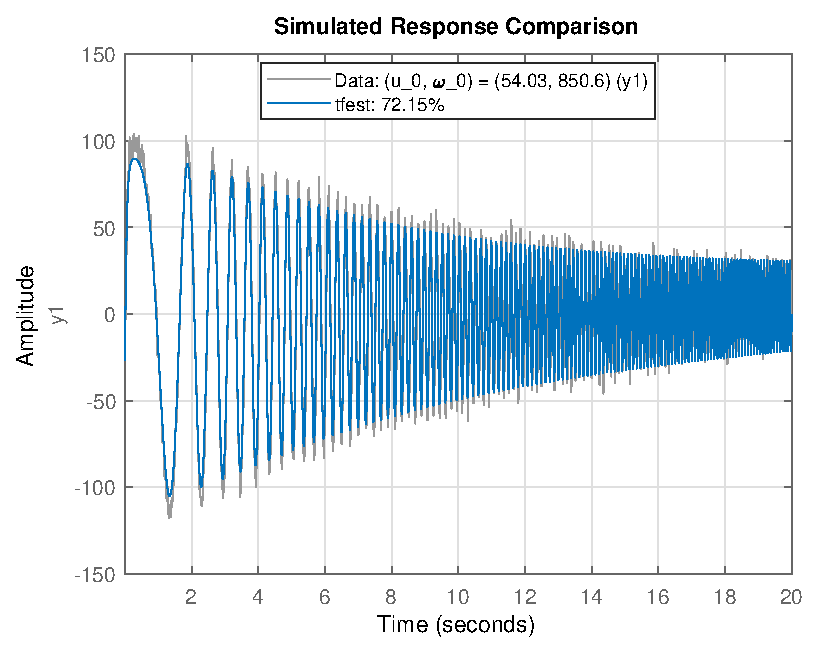
\includegraphics[width = \textwidth]{./figs/small_perturbation/time_Compare_1700.eps}
       \end{figure}
    \end{minipage}
    \begin{minipage}{0.32\textwidth}
       \begin{figure}[H]
            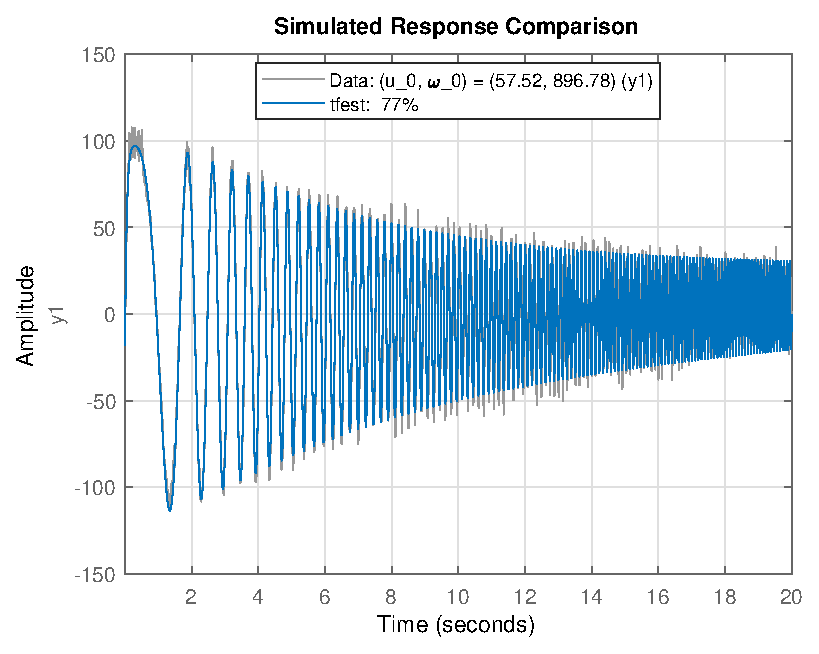
\includegraphics[width = \textwidth]{./figs/small_perturbation/time_Compare_1750.eps}
       \end{figure}
    \end{minipage}
\end{figure}


%===============================================================================
%\newpage
%===============================================================================
\newpage
\bibliographystyle{unsrt}
\bibliography{refs}

\end{document}
